\section{  FROM SCIENCE DRIVERS TO REFERENCE DESIGN}
\label{Sec:refdesign}

The most important characteristic that determines the speed at which a system can
survey a given sky area to a given flux limit (i.e., its depth) is its \'etendue
(or grasp), the product of its primary mirror area and the angular
area of its field of view (for a given set of observing conditions, such as
seeing and sky brightness).
The effective \'etendue for LSST will be greater than 300 m$^2$ deg$^2$, which
is more than an order of magnitude larger than that of any existing facility.
For example, the SDSS, with its 2.5-m telescope (Gunn et al.~2006) and a
camera with 30 imaging CCDs (Gunn et al.~1998), has an effective \'etendue of
only 5.9 m$^2$ deg$^2$.

The range of scientific investigations which will be enabled by such a
dramatic improvement in survey capability is extremely broad. Guided by
the community-wide input assembled in the report of the Science Working Group of the
LSST in 2004\footnote{Available as
http://www.lsst.org/files/docs/DRM2.pdf}, the LSST is designed to
achieve goals set by four main science themes:

\begin{enumerate}
\item Probing Dark Energy and Dark Matter;
\item Taking an Inventory of the Solar System;
\item Exploring the Transient Optical Sky;
\item Mapping the Milky Way.
\end{enumerate}

Each of these four themes itself encompasses a variety of analyses, with
varying sensitivity to instrumental and system parameters. These themes
fully exercise the technical capabilities of the system, such as photometric
and astrometric accuracy and image quality. About 90\% of the observing time
will be devoted to a deep-wide-fast (main) survey mode. The working paradigm is that all
scientific investigations will utilize a common database constructed from an optimized
observing program (the main survey mode), such as that discussed in
\S~\ref{sec:baseline}.
Here we briefly describe these science goals and the most challenging requirements for the
telescope and instrument that are derived from those goals, which will
inform the overall system design decisions discussed below.
For a more detailed discussion, we refer the reader to the LSST Science Requirements
Document\footnote{Available at
http://www.lsst.org/files/docs/SRD.pdf},
\B{the LSST Science Book}
%\footnote{Available at http://www.lsst.org/lsst/SciBook and as
%arXiv:0912.0201}
(2009; hereafter SciBook),
as well as to numerous LSST poster presentations at recent
meetings of the AAS\footnote{See
http://www.lsst.org/lsst/content/aas2013 and further links at
http://www.lsst.org/lsst/news .}.


\subsection{The Main Science Drivers }

The main science drivers are used to optimize various system parameters.
Ultimately, in this high-dimensional parameter space, there is a
manifold defined by the total project cost. The science
drivers must both justify this cost, as well as provide guidance
on how to optimize various parameters while staying within the cost envelope.

Here we summarize the dozen or so most important interlocking constraints on data
and system properties placed by the four main science themes:

\begin{enumerate}
\item  The depth of a single visit;
\item  Image quality;
\item  Photometric accuracy;
\item  Astrometric accuracy;
\item  Optimal exposure time;
\item  The filter complement;
\item  The distribution of revisit times (i.e., the cadence of observations),
                including the survey lifetime;
\item  The total number of visits to a given area of sky;
\item  The coadded survey depth;
\item  The distribution of visits on the sky, and the total sky coverage;
\item  The distribution of visits per filter; and
\item  Data processing and data access (e.g., time delay for reporting
         transient sources and the software contribution to measurement errors).
\end{enumerate}

We present a detailed discussion of how these science-driven data properties are
transformed to system parameters below.


\subsubsection{Probing Dark Energy and Dark Matter}
\label{sec:Dark_Energy}

Current models of cosmology require the existence of both dark matter and dark
energy to match observational constraints (Riess et al.~2007; Komatsu et al.~2009;
Percival et al.~2010; LSST Dark Energy Science Collaboration 2012, and
references therein). Dark energy affects the cosmic history of both the Hubble expansion
and mass clustering. Distinguishing competing models for the physical
nature of dark energy, or alternative explanations involving
modifications of the General Theory of Relativity, will require
percent level measurements of both the cosmic expansion and the growth
of dark matter structure as a function of redshift.  Any given
cosmological probe is sensitive to, and thus constrains degenerate
combinations of, several cosmological parameters.  Therefore the most robust
cosmological constraints are the result of using interlocking combinations
of probes. The most powerful probes include weak gravitational lens cosmic shear (WL), galaxy clustering and baryon
acoustic oscillations (LSS),
the mass function of clusters of galaxies,
time delays in lensed quasar and supernova systems (SL),
and photometry of type Ia supernovae (SN) -- all as functions of
redshift. Using the cosmic microwave background fluctuations as the normalization, the
combination of these probes can yield the needed precision to distinguish among models of dark
energy (see e.g. Zhan 2006, and references therein). The challenge is to turn this available precision into accuracy, by careful modeling and marginlization over a variety of systematic effects (see e.g. Krause \& Eifler 2017).

Meanwhile, there are a number of astrophysical probes of the fundamental
properties of dark matter worth exploring, including, for example, merging
galaxy clusters (see e.g., Dawson et al.~2012) and mass density profiles in
clusters and galaxies (both accessible through their weak and strong lensing
effects in combination with measurments of their dynamics, stellar mass, and
X-ray emission; Newman et al.~2013 and Rocha et al.~2012), dwarf satellite
galaxies (both their abundance and gamma ray emission; see e.g., Hargis et
al.~2014 and Drlica-Wagner et al.~2015),  the subtle perturbations of stellar
streams (Belokurov \& Koposov 2016), and massive compact halo object
microlensing (Alcock et al.~2001).

Three of the primary Dark Energy probes, WL, LSS and SN,  provide unique and
independent constraints on the system design (SciBook Ch.~11--15).

Weak lensing (WL) techniques can be used to map the distribution of
mass as a function of redshift and thereby trace the history of both
the expansion of the Universe and the growth of structure (e.g., Hu \&
Tegmark 1999; for reviews see Bartelmann \& Schneider 2001 and
Weinberg et al.~2013).  Measurements of cosmic shear as a function of
redshift allow determination of angular distances versus cosmic time,
providing multiple independent constraints on the nature of dark
energy.  These investigations require deep wide-area multi-color
imaging with stringent requirements on shear systematics in at least
two bands, and excellent photometry in at least five bands to measure
photometric redshifts (a requirement shared with LSS, and indeed all
extragalactic science drivers). The strongest constraints on the LSST
image quality arise from this science program. In order to control
systematic errors in shear measurement, the desired depth must be
achieved with many short exposures (allowing for systematics in the
measurement of galaxy shapes related
to the PSF and telescope pointing to be diagnosed and removed). Detailed simulations of
weak lensing techniques show that imaging over $\sim20,000$ deg$^2$ to
a 5$\sigma$ point-source depth of $r_{AB} \sim 27.5$ gives adequate
signal to measure shapes for of order 4 billion galaxies for weak
lensing.  These numbers are adequate to reach
Stage IV goals for dark energy, as defined by the Dark Energy Task
Force (Albrecht et al.~2006).
This
depth, \B{and the corresponding deep surface brightness limit,}
optimize the number of galaxies with measured shapes in ground-based
seeing, and allow their detection in significant numbers to beyond a
redshift of two.  Analyzing these data will
require sophisticated data processing techniques.  For example, rather
than simply coadding all images in a given region of sky, the
individual exposures, each with their own PSF and noise
characteristics,  should be analyzed simultaneously to optimally
measure the shapes of galaxies (Tyson et al.~2008a;
Jee and Tyson, 2011).

Type Ia supernovae provided the first robust evidence that the expansion of the
Universe is accelerating (Riess et al.~1998; Perlmutter et al.~1999). To fully
exploit the supernova science potential, light curves sampled in multiple
bands every few days over the course of a few months are required. This is
essential to search for systematic differences in supernova populations
(e.g., due to differing progenitor channels) which
may masquerade as cosmological effects, as well as to determine photometric
redshifts from the supernovae themselves. Unlike other cosmological probes,
even a single object gives information on the relationship between
redshift and distance.  Thus a large
number of SN across the sky allows one to search for any dependence
of dark energy properties on direction, which
would be an indicator of new physics. The results from this method can be compared
with similar measures of anisotropy from the combination of WL and LSS
(Zhan et al.~2009).
Given the expected SN flux distribution
at the redshifts where dark energy is important, the
single visit depth should be at least $r\sim24$. Good image quality is
required to separate SN photometrically from
their host galaxies. Observations in at least five photometric bands will allow
proper K-corrected light curves to be measured over a range of
redshift.  Carrying out these K-corrections requires that the
calibration of the relative offsets in photometric zero points between filters and
the system response functions, especially near the edges of
bandpasses, must be accurate to about 1\% (Wood-Vasey et al.~2007),
similar to the requirements from photometric redshifts of galaxies. Deeper data
($r>26$) for small areas of the sky can extend the discovery of SN to a mean
redshift of 0.7 (from $\sim0.5$ for the main survey), with some objects beyond $z\sim$1
(Garnavich et al.~2005; Pinto et al.~2005; SciBook Ch.~11). The added statistical leverage
on the ``pre-acceleration'' era ($z\ga1$) would improve constraints on the properties of
dark energy as a function of redshift.

Finally, there will be powerful cross checks and complementarities with other planned or
proposed surveys, such as Euclid (Laureijs et al.~2011) and WFIRST-AFTA
(Spergel et al.~2013)
%\footnote{http://wfirst.gsfc.nasa.gov}
(wide-field optical-IR imaging from space),
DESI (Levi et al.~2013)
%\footnote{http://desi.lbl.gov}
and PFS (Takada et al.~2014)
(spectroscopic BAO with several
millions of galaxies), and SKA\footnote{https://www.skatelescope.org} (radio).
Large survey volumes are key to probing dynamical dark energy models (with sub-horizon
dark energy clustering or anisotropic stresses). The cross-correlation
of the three-dimensional
mass distribution (as probed by HI in SKA, or galaxies in DESI and PFS) with the gravitational growth
probed by tomographic shear in LSST will be complementary way to constrain dark energy
properties beyond simply characterizing its equation of state.



\subsubsection{Taking an Inventory of the Solar System}


The small-body populations in the Solar System, such as asteroids, trans-Neptunian objects (TNOs)
and comets, are remnants of its early assembly. The history of accretion, collisional grinding, and
perturbation by existing and vanished giant planets is preserved in the orbital elements and size
distributions of those objects. Cataloging the orbital parameters, size distributions, colors and light
curves of these small-body populations requires a large number of observations in multiple filters,
and will lead to insights into planetary formation and evolution by providing the basis and constraints
for new theoretical models. In addition, collisions in the main asteroid belt between Mars and Jupiter
still occur, and occasionally eject objects on orbits that may place them on a collision course with Earth.
Studying the properties of main belt asteroids at sub-kilometer sizes is important for linking the near-Earth
Object (NEO) population with its source in the main belt. About 20\% of NEOs, the potentially hazardous
asteroids (PHAs), are in orbits that pass sufficiently close to Earth's orbit, to within 0.05 AU, that perturbations
with time scales of a century can lead to intersections and the possibility of collision. In December 2005,
the U.S. Congress directed\footnote{For details see http://neo.jpl.nasa.gov/neo/report2007.html} NASA to
implement a NEO survey that would catalog 90\% of NEOs with diameters larger than 140 meters by 2020.

Discovering and linking objects in the Solar System moving with a wide range of apparent velocities (from
several degrees per day for NEOs to a few arc seconds per day for the most distant TNOs) places strong
constraints on the cadence of observations, requiring closely spaced pairs of observations (two or preferably
three times per lunation) in order to link detections unambiguously and derive orbits (SciBook Ch.~5). Individual
exposures should be shorter than about 30 seconds each to minimize the effects of trailing for the majority of
moving objects. The images must be well sampled to enable accurate astrometry, with absolute accuracy of at
least 0.1 arcsec in order to measure orbital parameters of TNOs with enough precision to constrain theoretical
models and enable prediction of occulations. The photometry should be
better than 1-2\% to measure asteroids' colors and thus determine
their types.  The different filters
should be observed over a short time span to reduce apparent
variations in color due to changes in observing geometry, but should
be repeated over many lunations in order to determine phase curves and allow shape modeling.

The Congressional mandate can be fulfilled with a 10-meter-class
telescope equipped with a multi-gigapixel camera, and a sophisticated
and robust data processing system (Ivezi\'{c} et al.~2007a). The images should reach a depth of at
least 24.5 (5$\sigma$ for point sources) in the $r$ band to reach high
completeness down to the 140 m mandate for NEOs.  Such an instrument
would probe the $\sim$100 m size range at main-belt distances, and
discover rare distant TNOs such as Sedna (Brown, Trujillo \&
Rabinowitz 2004) and 2012 VP113 (Trujillo \& Sheppard 2014).


\subsubsection{ Exploring the Transient Optical Sky}

Recent surveys have shown the power of measuring variability for
studying gravitational lensing, searching for supernovae, determining
the physical properties of gamma-ray burst sources, discovering
gravitational wave counterparts, probing the structure of active
galactic nuclei, studying variable star populations, discovering
exoplanets, and many other subjects at the forefront of astrophysics
(SciBook Ch.~8; Law et al.~2009; Djorgovski et al.~2012; Rowe et
al.~2014).

Time-domain science has diverse requirements for transient and
variable phenomena that are physically and phenomenologically
different: it requires large area coverage to enhance the probability
of detecting rare events; good image quality to enable differencing of
images, especially in crowded fields; good time sampling, necessary to
distinguish different types of variables and in some cases to infer
their properties (e.g. determining the intrinsic luminosity of Type Ia
supernovae depends on measurements of their rate of decline); accurate
color information to assist with the classification of variable
objects (e.g., to reduce microlensing and kilonova false positives;
note that this requirement may be in tension with the dense sampling requirement); long term
persistent observations to characterize slow-evolving transients
(e.g. tidal disruption events, super luminous supernovae at high
redshift, and luminous blue variables); and rapid data reduction,
classification, and reporting to the community in order to flag
interesting targets for spectroscopic follow-up, as well as
photometric follow-up in optical wavebands to collect denser time
series and in other wavebands.

Wide area, dense temporal coverage to deep limiting magnitudes will
enable the discovery and analysis of rare and exotic objects such as
neutron stars and black hole binaries, novae and stellar flares,
gamma-ray bursts and Xray flashes, active galactic nuclei, stellar
disruptions by black holes (Bloom et al. 2011; Gezari et al. 2012),
and possibly new classes of transients, such as binary mergers of
black holes (Shields \& Bonning 2008; Thornton et al. 2013) and chaotic
eruptions (Arnett \& Meakin 2011), and, further yet, completely
unexpected phenomena.

Such a survey would likely detect microlensing by stars and compact objects in
the Milky Way, but also in the Local Group and perhaps beyond (de Jong, Kuijken
\& H\'{e}raudeau 2008). Given the duration of the LSST it will also be possible
to detect the parallax microlensing signal of intermediate mass black holes and
measure their mass (Gould 1992). It would open the possibility of
discovering populations of binaries and planets via transits (e.g., Beaulieu et
al.~2006; Drake et al.~2010; Choi et al.~2013; Batista et al.~2014), as well as
obtaining spectra of lensed stars in distant galaxies.

A deep and persistent survey will discover precursors of explosive and
eruptive transients, generate large samples of transients whose study
has thus far been limited by small sample size (e.g. different
subtypes of core collapse SN, Bianco et al.~2014.)

Time series ranging between one minute and ten years cadence should be
probed over a significant fraction of the sky. The survey's cadence
will be sufficient, combined with the large coverage, to
serendipitously catch very short-lived events, such as eclipses in
ultra-compact double degenerate binary systems (Anderson et al.~2005),
to constrain the properties of fast faint transients (such as optical
flashes associated with gamma-ray bursts; Bloom et al.~2008), to
detect electromagnetic counterparts to gravitational waves (Nissanke,
Kasliwal \& Georgieva~2013, Scolnic~2017) and to further constrain the
properties of new classes of transients discovered by programs such as
the Deep Lens Survey (Becker et al.~2004), the Catalina Real-time
Transient Survey (Drake et al.~2009) and the Palomar Transient Factory
(Law et al~ 2009), the Zwicky Transient Factory (Bellm~2014). Observations
over a decade will enable the study of long period variables, intermediate mass
black holes, and quasars (Kaspi et al. 2007; MacLeod et al. 2010; Graham et al.
2014; Chapline \& Frampton 2016).


The next frontier
in this field will require measuring the colors of fast transients,
and to probe variability at faint magnitudes. Classification of transients in
close-to-real time will require access to the full photometric history
of the objects, both before and after the transient event (e.g.,
Mahabal et al.~2011).


%\vskip 0.5in
\subsubsection{ Mapping the Milky Way}

A major challenge in extragalactic cosmology today concerns the formation of structure on sub-galactic scales, where
baryon physics becomes important, and the nature of dark matter may manifest itself in observable ways (e.g., Weinberg
et al.~2013). The Milky Way and its environment provide a unique dataset for understanding the detailed processes that
shape galaxy formation and for testing the small-scale predictions of
our standard cosmological model. However, we still lack
answers to two basic questions about our Galaxy:
\begin{itemize}
\item What is the detailed structure and accretion history of the Milky Way?
\item What are the fundamental properties of all the stars within 300 pc of the Sun?
\end{itemize}

Mapping the Galaxy requires large area coverage, excellent image
quality to maximize photometric and astrometric accuracy,
especially in crowded fields, photometric precision of at least 1\% to
separate main sequence and
giant stars (e.g., Helmi et al.~2003) as well as to identify variable
stars such as RR Lyrae (Sesar et al.~2010, Sharma et al.~2011),
and astrometric precision of about 10 mas per observation to enable parallax and proper motion measurements
(SciBook Ch.~6,7). In order to probe the halo out to its presumed edge at $\sim100$ kpc (Ivezi\'{c} et al.~2003) using
main-sequence stars, the total coadded depth must reach $r > 27$, with a similar depth in the $g$ band.
The metallicity distribution of stars can be studied photometrically in the Sgr tidal stream (e.g., see
Majewski et al.~2003, Chou et al.~2007) and other halo substructures
($\sim 30$ kpc, Carollo et al.~2007), yielding new insights into how
they formed.  These
metallicities are limited by the coadded depth in the $u$ band.  To reach the limit of the stellar halo, this must reach
$u\sim24.5$. To detect RR Lyrae stars beyond the Galaxy's tidal radius at $\sim 300$ kpc, the single-visit depth must
be $r \sim  24.5$.

In order to measure the tangential velocity of stars at a distance of 10 kpc, where the halo dominates over the disk, to
within 10 km s$^{-1}$ (comparable with the accuracy of
large-scale radial velocity surveys), the proper motion
accuracy should be 0.2 mas yr$^{-1}$ or better. This is the same accuracy as will be delivered by the recently launched Gaia mission\footnote{http://sci.esa.int/gaia/} (Perryman et al.~2001; de Bruijne 2012) at its faint limit ($r \sim 20$).
In order to measure distances to solar neighborhood stars out to a distance of 300 pc (the thin disk scale height),
with geometric distance accuracy of at least 30\%, trigonometric parallax measurements accurate to 1 mas ($1\sigma$)
are required over 10 years. To achieve the required proper motion and parallax accuracy with an assumed astrometric
accuracy of 10 mas per observation per coordinate, approximately 1,000
separate observations are required. This requirement for a large
number of observations is in good agreement with that from minimizing
systematics in weak lensing observations (\S~\ref{sec:Dark_Energy}).


%\subsubsection{A Summary and Synthesis of Science-driven Constraints on Data Properties}

\begin{figure}
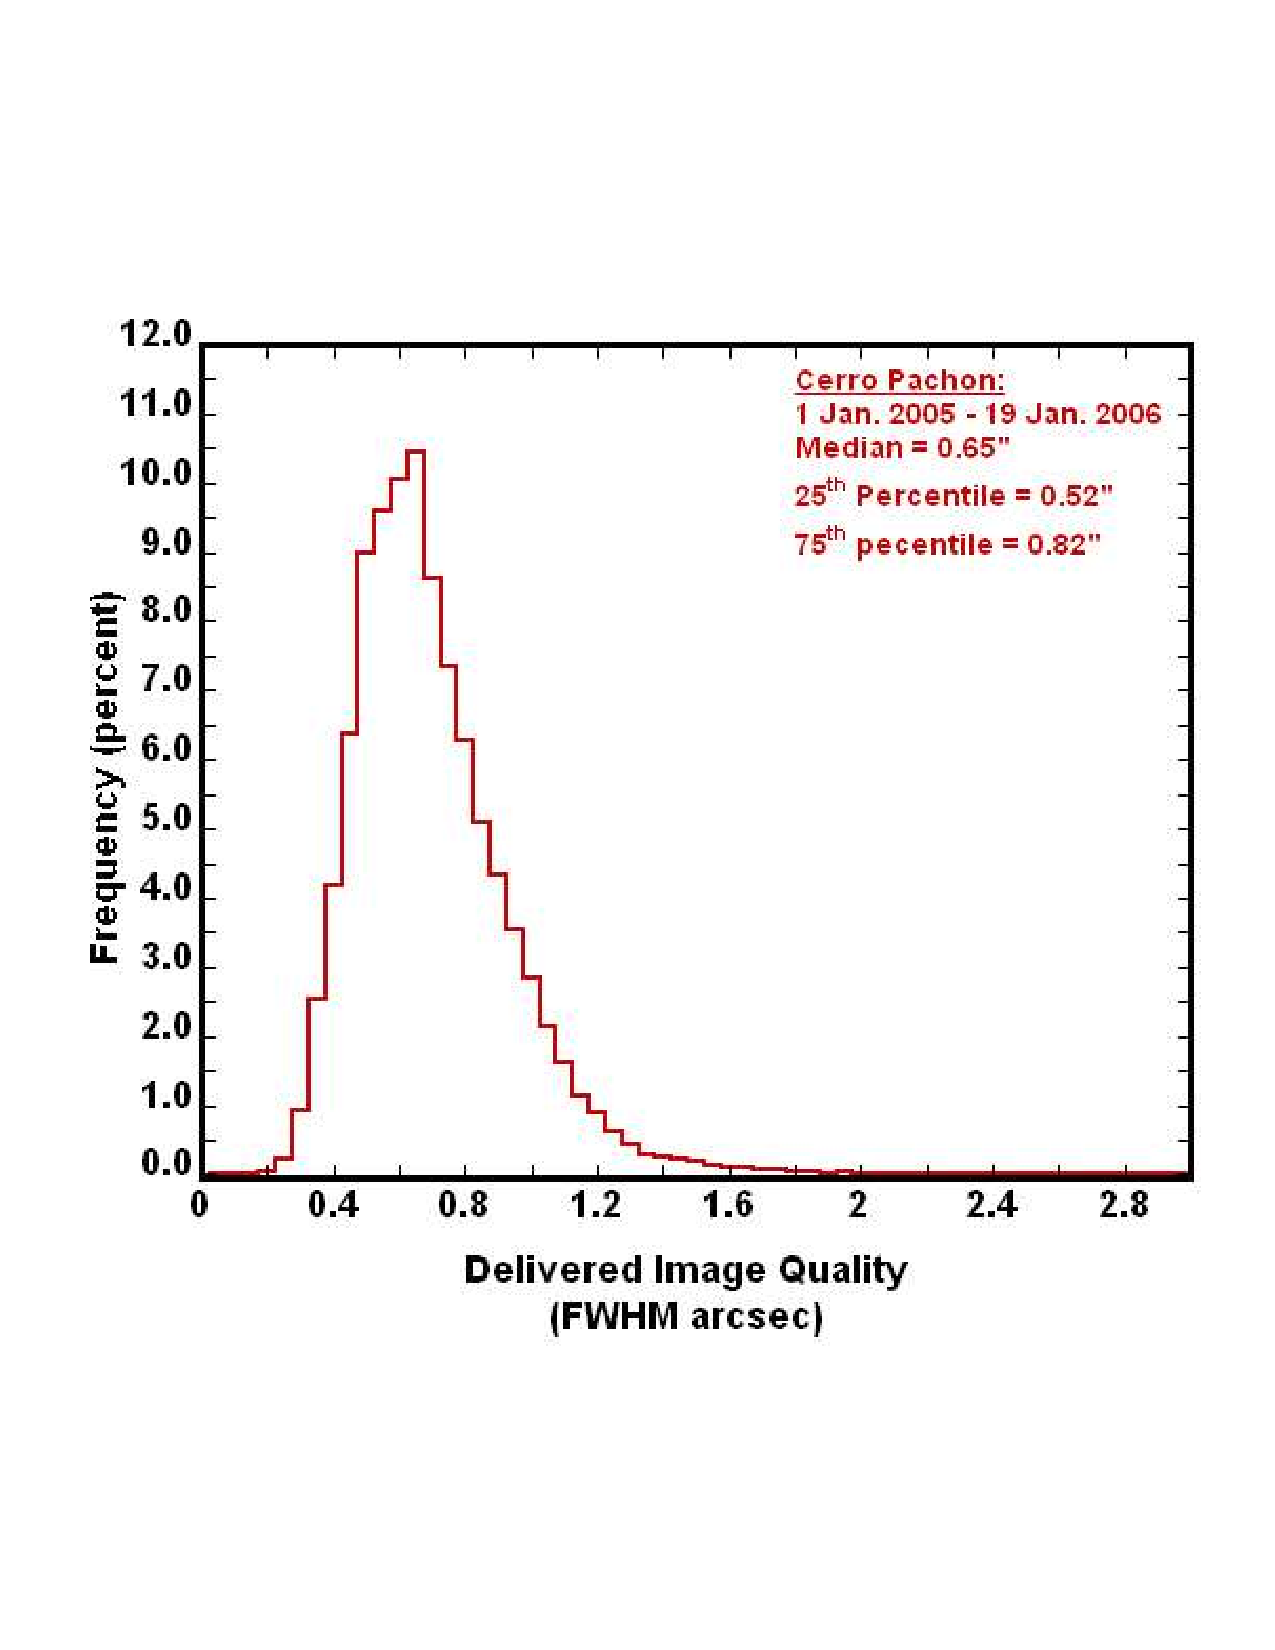
\includegraphics[width=1.0\hsize,clip]{seeing2.pdf}
\caption{
The image quality distribution measured at the Cerro Pach\'{o}n site using
a differential image motion monitor (DIMM) at $\lambda$ = 500 nm, and corrected
using an outer scale parameter of 30 m over an 8.4 m aperture. For details
about the outer scale correction see Tokovinin (2002). The observed distribution
is well described by a log-normal distribution, with the parameters shown in
the figure.}
\label{Fig:seeing}
\end{figure}

\subsubsection{A Summary and Synthesis of Science-driven Constraints on Data Properties}

The goals of all the science programs discussed above
(and many more, of course) can be accomplished by satisfying the
minimal constraints listed below. For a more elaborate listing
of various constraints, including detailed specification of
various probability density distribution functions, please see the LSST Science
Requirements Document\footnote{http://www.lsst.org/files/docs/SRD.pdf}
and the LSST Science Book.

\begin{enumerate}
\item  {\it The single visit depth} should reach $r\sim24.5$. This limit is
   primarily driven by the search for NEOs, variable sources (e.g., SN,
   RR Lyrae stars), and by proper motion and trigonometric parallax
   measurements for stars. Indirectly, it is also driven by the
   requirements on the coadded survey depth and the minimum number of
   exposures required by WL science.  We will split a single visit
   into two exposures of equal length to identify and remove cosmic
   rays.
\item  {\it Image quality} should maintain the limit set by the
     atmosphere (the median free-air seeing is 0.65 arcsec in the $r$ band
     at the chosen site, see Fig.~\ref{Fig:seeing}),
     and not be degraded appreciably by the hardware. In addition to stringent
     constraints from weak lensing, good image quality is driven by the
     required survey depth for point sources and by image differencing
     techniques.
\item  {\it Photometric repeatability} should achieve 5 mmag precision
     at the bright end, with zeropoint stability across the sky of 10 mmag
     and band-to-band calibration errors not larger than 5 mmag.
     These requirements are driven by the need for high photometric redshift accuracy,
     the separation of stellar populations, detection of low-amplitude variable
     objects (such as eclipsing planetary systems), and the search for
     systematic effects in type Ia supernova light curves.
\item  {\it Astrometric precision} should maintain the limit set by
     the atmosphere, of about 10 mas per visit at the bright end
     (on scales below 20 arcmin). This precision is driven by the desire to
     achieve a proper motion accuracy of 0.2 mas yr$^{-1}$ and parallax accuracy of
     1.0 mas over the course of a 10-year survey (see \S \ref{sec:astrom}).
\item  {\it The single visit exposure time} (including both exposures in a
    visit, which are required for cosmic ray rejection) should be less than about a minute
    to prevent trailing of fast moving objects and to aid control
    of various systematic effects induced by the atmosphere. It should
    be longer than $\sim$20 seconds to avoid significant efficiency losses due to
    finite readout, slew time, and read noise.
\item  {\it The filter complement} should include at least six filters
    in the wavelength range limited by atmospheric absorption and
    silicon detection efficiency (320--1050 nm), with roughly
    rectangular filters and no large gaps in the coverage, in order
    to enable robust and accurate photometric redshifts and stellar typing. An
    SDSS-like $u$ band (Fukugita et al.~1996) is extremely important for separating
    low-redshift quasars from hot stars, and for estimating the metallicities of
    F/G main sequence stars. A bandpass with an effective wavelength of
    about 1 micron  would enable studies of sub-stellar objects, high-redshift
    quasars (to redshifts of $\sim$7.5), and regions of the Galaxy that are obscured
    by interstellar dust.
\item  {\it The revisit time distribution} should enable determination of
   orbits of Solar System objects and sample SN light curves every few days,
   while accommodating constraints set by proper motion and trigonometric
   parallax measurements.
\item  {\it The total number of visits} of any given area of sky, when accounting for all
   filters, should be of the order of 1,000, as mandated by WL
   science, the search for NEOs, and proper motion and
   trigonometric parallax measurements. Studies of transient sources
   also benefit from a large number of visits.
\item  {\it The coadded survey depth} should reach
    $r\sim27.5$, with sufficient signal-to-noise ratio in other bands
    to address both extragalactic and Galactic science drivers.
\item  {\it The distribution of visits per filter} should enable
   accurate photometric redshifts, separation of stellar populations,
   and sufficient depth to enable detection of faint extremely red
   sources (e.g., brown dwarfs and high-redshift quasars). Detailed simulations of
   photometric redshift estimates
   suggest an approximately flat distribution of visits among bandpasses
   (because the system throughput and atmospheric properties are
    wavelength dependent, the achieved depths are different in different
    bands). The adopted time allocation
   (see Table 1) includes a slight preference to the $r$ and $i$ bands because of their
   dominant role in star/galaxy separation and weak lensing measurements.
\item  {\it The distribution of visits on the sky} should extend over
   at least $\sim$20,000 deg$^2$ to obtain the required number of galaxies
   for WL studies, with attention paid to include ``special''
   regions such as the Ecliptic and Galactic planes, and the Large and Small
   Magellanic Clouds (if in the Southern Hemisphere).  Note that
   20,000 deg$^2$ is comparable to the full area observable from any
   given ground-based site at reasonably low airmass (the LSST survey area will
   be contained within 30,000 deg$^2$ with $\delta<+34.5^\circ$).
\item  {\it Data processing, data products and data access} should
  result in data products that approach the statistical uncertainties
  in the raw data; i.e., the processing must be close to optimal.
%enable efficient science analysis without a significant impact on the
%final uncertainties.
To enable fast and efficient response to
   transient sources, the processing latency for variable sources should be less than a minute,
   with a robust and accurate preliminary characterization
   %classification
   of all reported variables.
\end{enumerate}

Remarkably, even with these joint requirements, none of the
individual science programs is severely over-designed, i.e., despite
their significant scientific diversity, these programs are highly
compatible in terms of desired data characteristics. Indeed, any one
of the four main science drivers could be removed, and the remaining
three would still yield very similar requirements for most system
parameters. As a result, the LSST system can adopt a highly
efficient survey strategy where {\it a single dataset serves most science
programs} (instead of science-specific surveys executed in series).
One can view this project as {\it massively parallel astrophysics}.
The vast majority (about 90\%) of the observing time will be devoted to
a deep-wide-fast survey mode, with the remaining 10\%
allocated to special programs which will also address multiple science
goals. Before describing these surveys in detail, we discuss the main
system parameters.


\begin{table}
\caption{The LSST Baseline Design and Survey Parameters}
\begin{tabular}{|l|l|}
\hline
   Quantity                         &     Baseline Design Specification    \\
\hline
Optical Config.                           &  3-mirror modified Paul-Baker        \\
Mount Config.                            &  Alt-azimuth          \\
Final f-ratio, aperture                 &  f/1.234, 8.4 m                \\
Field of view, \'etendue              &  9.6 deg$^2$,   319 m$^2$deg$^2$     \\
Plate Scale                                  &  50.9 $\mu$m/arcsec (0.2'' pix)  \\
Pixel count                                  &  3.2 Gigapix  \\
Wavelength Coverage                   &  320 -- 1050 nm, $ugrizy$             \\
Single visit depths, design $^a$  &  23.9, 25.0, 24.7, 24.0, 23.3, 22.1    \\
Single visit depths, min.$^b$       &  23.4, 24.6, 24.3, 23.6, 22.9, 21.7    \\
Mean number of visits$^c$          &  56, 80, 184, 184, 160, 160               \\
Final (coadded) depths$^d$         &  26.1, 27.4, 27.5, 26.8, 26.1, 24.9     \\
\hline
\end{tabular}
\\ \vskip 0.05in
$^a$ Design specification from the Science Requirements Document (SRD) for 5$\sigma$ depths
for point sources in the $ugrizy$ bands, respectively. The listed values are expressed on AB magnitude
scale, and correspond to point sources and fiducial zenith observations (about 0.2 mag loss of depth
is expected for realistic airmass distributions, see Table 2 for more details).
$^b$ Minimum specification from the Science Requirements Document for 5$\sigma$ depths.
$^c$ An illustration of the distribution of the number of visits as a function of bandpass,
taken from Table 24 in the SRD.
$^d$ Idealized depth of coadded images, based on design specification for 5$\sigma$ depth and
the number of visits in the penultimate row (taken from Table 24 in the SRD).
\vskip 0.2in
\end{table}



\subsection{The Main System Design Parameters}

Given the minimum science-driven constraints on the data properties listed
in the previous section, we now discuss how they are translated into
constraints on the main system design parameters: the aperture size,
the survey lifetime, the optimal exposure time, and the filter complement.


\subsubsection{ The Aperture Size }
\label{Sec:apSize}
The product of the system's \'etendue and the survey lifetime, for given
observing conditions, determines
the sky area that can be surveyed to a given depth.
%, where the \'etendue is the product of the primary mirror area and
%the field-of-view area.
The
LSST field-of-view area is maximized to its practical limit, $\sim$10 deg$^2$,
determined by the requirement that the delivered image quality be dominated
by atmospheric seeing at the chosen site (Cerro Pach\'{o}n in Northern Chile).
A larger field-of-view would lead to unacceptable deterioration of the
image quality. This constraint leaves the primary mirror diameter and survey lifetime
as free parameters. The adopted survey lifetime of 10 years is a compromise
between a shorter time that leads to an excessively large and expensive mirror (15 m for a
3 year survey and 12 m for a 5 year survey) and not as effective proper motion
measurements, and a smaller telescope that would require more time to complete the
survey, with the associated increase in operations cost.

The primary mirror size is a function of the required survey depth and the
desired sky coverage. By and large, the anticipated science outcome scales
with the number of detected sources. For practically all astronomical source
populations, in order to maximize the number of detected sources, it is more
advantageous to maximize the area first, and then
the detection depth\footnote{
If the total exposure time is doubled and used to double the survey area,
the number of sources increases by a factor of two. If the survey
area is kept fixed, the increased exposure time will result in
$\sim$0.4 mag deeper data (see eq.~\ref{m5}). For cumulative source
counts described by $\log(N) = C + k*m$, the number of sources
will increase by more than a factor of two only if $k>0.75$.
Apart from $z<2$ quasars, practically all populations
have $k$ at most 0.6 (the Euclidean value), and faint stars
and galaxies have $k<0.5$. For more details, please see Nemiroff
(2003).}. For this reason, the sky area for the main survey is
maximized to its practical limit, 18,000 deg$^2$, determined by the
requirement to avoid airmasses less than 1.5,
%$X<1.5$, where approximately $X={\rm sec}(\theta)$  and $\theta$ is
%the zenith distance),
which would substantially
deteriorate the image quality and the survey depth (see eq.~\ref{m5}).

With the adopted field-of-view area, the sky coverage and the survey lifetime
fixed, the primary mirror diameter is fully driven by the required survey
depth. There are two depth requirements: the final (coadded) survey depth,
$r\sim27.5$, and the depth of a single visit, $r\sim24.5$. The two
requirements are compatible if the number of visits is several hundred
per band, which is in good agreement with independent science-driven
requirements on the latter.

The required coadded survey depth provides a direct constraint,
independent of the details of survey execution such as the exposure time per visit,
on the minimum effective primary mirror diameter of 6.5 m, as illustrated in
Fig.~\ref{Fig:coaddDepth}.



\subsubsection{ The Optimal Exposure Time }

The single visit depth depends on both the primary mirror diameter and the
chosen exposure time, $t_{\rm vis}$. In turn, the exposure time
determines the time interval to revisit a given sky position and the total
number of visits, and each of these quantities has its own science
drivers. We summarize these simultaneous constraints in terms of the
single-visit exposure time:
\begin{itemize}
\item  The single-visit exposure time should not be longer than about a minute to
         prevent trailing of fast Solar System moving objects, and to enable efficient
         control of atmospheric systematics.
\item  The mean revisit time (assuming uniform cadence) for a given position
         on the sky, $n$, scales as
\begin{equation}
  n = \left( {t_{\rm vis} \over 10  \, {\rm sec}} \right)
      \left( { A_{\rm sky} \over 10,000  \, {\rm deg}^2} \right)
      \left( {10 \, {\rm deg}^2 \over  A_{\rm FOV}} \right) {\rm days},
\end{equation}
where two visits per night are assumed (required for efficient detection of
Solar System objects, see below), and the losses for realistic observing conditions
have been taken into account (with the aid of the Operations Simulator described below).
Science drivers such as supernova light curves and moving objects in the Solar System require
that $n<4$ days, or equivalently $t_{vis} < 40$ seconds for the nominal values
of $A_{sky} $ and $A_{FOV}$.
\item  The number of visits to a given position on the sky, $N_{visit}$,
%again
with losses for realistic observing conditions taken into account,
is given by
\begin{equation}
      N_{visit} = \left( {3000 \over n} \right)
                    \left( { T \over 10 \, {\rm yr}} \right).
\end{equation}
The requirement $N_{visit}>800$ again implies that $n<4$ and
$t_{vis} < 40$ seconds if the survey lifetime, $T \sim 10$ years.
\item  These three requirements place a firm upper limit on the
optimal visit exposure time of $t_{vis} < 40$ seconds. Surveying
efficiency (the ratio of open-shutter time to the total
time spent per visit) considerations place a lower limit on
$t_{vis}$ due to finite detector read-out and telescope slew time (the longest
acceptable read-out time is set to 2 seconds, the shutter open-and-close
time is 2 seconds, and the slew and settle time is set to 5 seconds, including
the read-out time for the second exposure in a visit):
\begin{equation}
      \epsilon = \left( {t_{vis} \over t_{vis} + 9 \, {\rm sec}}\right).
\end{equation}
To maintain efficiency losses below $\sim$30\% (i.e., at least below the
limit set by the weather patterns), and to minimize the read noise
impact, $t_{vis} > 20$ seconds is required.
\end{itemize}

Taking these constraints simultaneously into account, as summarized in
Fig.~\ref{Fig:singleDepth},
yielded the following reference design:
\begin{enumerate}
\item A primary mirror effective diameter of $\sim$6.5 m. With the adopted optical
design, described below, this effective diameter corresponds to a geometrical diameter
of $\sim$8 m. Motivated by characteristics of the existing equipment at the
Steward Mirror Laboratory, which is fabricating the primary mirror, the adopted
geometrical diameter is set to 8.4 m.
\item A visit exposure time of 30 seconds (using two 15 second exposures
to efficiently reject cosmic rays), yielding $\epsilon=77$\%.
\item A revisit time of 3 days on average for 10,000 deg$^2$ of sky,
  with two visits per night.
\end{enumerate}

\begin{figure}[t]
\vskip -0.5in
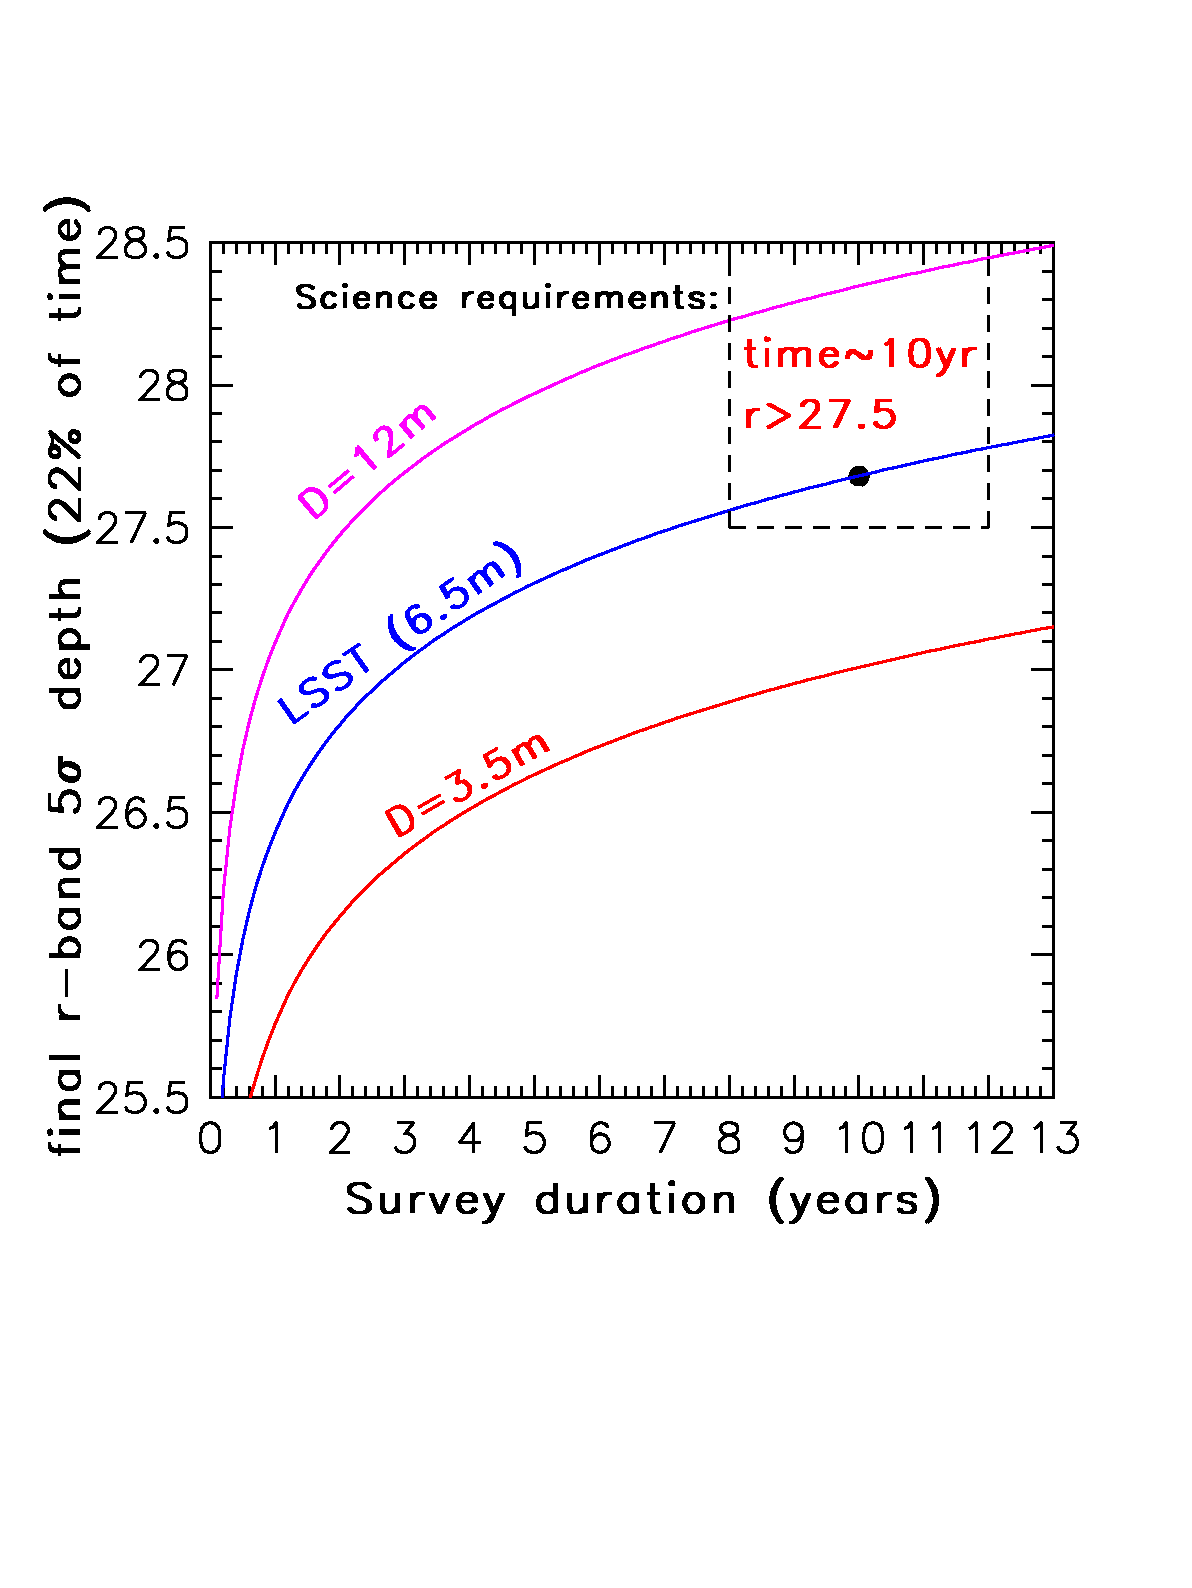
\includegraphics[width=1.1\hsize,clip]{coaddedDepth.pdf}
\vskip -1.1in
\caption{The coadded depth in the $r$ band (AB magnitudes) vs. the effective aperture and
the survey lifetime. It is assumed that 22\% of the total observing time (corrected for
weather and other losses) is allocated for the $r$ band, and that the ratio of
the surveyed sky area to the field-of-view area is 2,000.}
\label{Fig:coaddDepth}
\end{figure}

\begin{figure}[t]
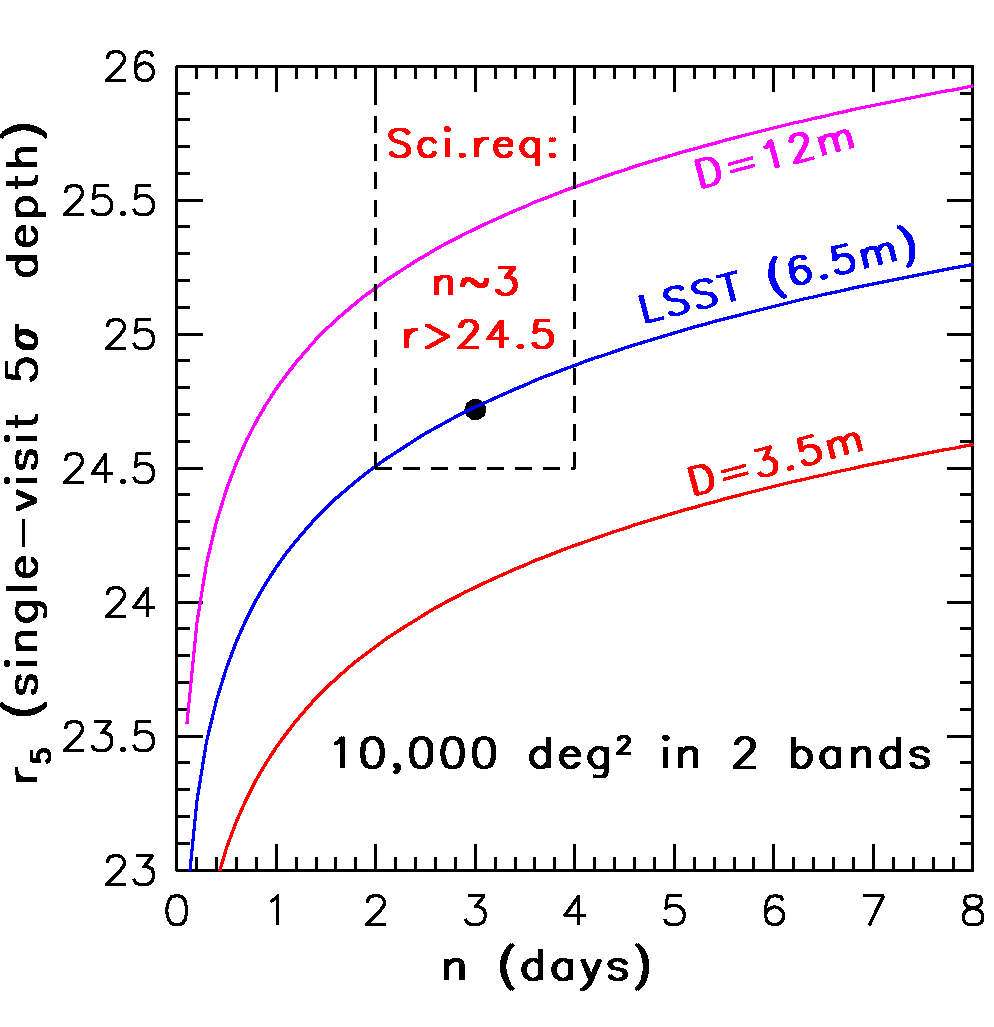
\includegraphics[width=1.0\hsize,clip]{singleDepth.pdf}
\caption{The single-visit depth in the $r$ band (5$\sigma$ detection for
point sources, AB magnitudes) vs. revisit time, $n$ (days), as a function of
the effective aperture size. With a coverage of 10,000 deg$^2$ in two bands,
the revisit time directly constrains the visit exposure time, $t_{vis}=10\,n$
seconds. In addition to direct constraints on optimal exposure time, $t_{vis}$
is also driven by requirements on the revisit time, $n$, the total number of visits
per sky position over the survey lifetime, $N_{visit}$, and the survey efficiency,
$\epsilon$ (see eqs.1-3). Note that these constraints result in a fairly narrow range of
allowed $t_{vis}$ for the main deep-wide-fast survey.}
\label{Fig:singleDepth}
\end{figure}

To summarize, the chosen primary mirror diameter is the {\it minimum}
diameter that simultaneously satisfies the depth ($r\sim24.5$ for single visit and
$r\sim27.5$ for coadded depth) and cadence (revisit time of 3-4 days,
with 30 seconds per visit) constraints described above.

\subsection{System Design Trade-offs}

We note that the Pan-STARRS project (Kaiser et al.~2002), with similar science
goals as LSST, has adopted a distributed aperture design, where the total
system \'etendue is
a sum of \'etendue values for an array of small telescopes (the prototype
PS1 telescope has an \'etendue 1/24$^{th}$ that of LSST).
Similarly, the LSST system could perhaps be made as two smaller copies with
6m mirrors, or 4 copies with 4m mirrors, or 16 copies with 2m mirrors. Each
of these clones would have to have its own 3 Gigapixel camera (see below), and
given the added risk and complexity (e.g., maintenance, data processing), the monolithic
design seems advantageous for a system with such a large \'etendue as LSST.

It is informative to consider the tradeoffs that would be required
for a system with a smaller aperture, if the science requirements were
to be maintained. For this comparison, we consider a four-telescope version of
the Pan-STARRS survey (PS4). With an \'etendue about 6 times smaller
than that of LSST (effective diameters of 6.5 m and 3.0 m, and a field-of-view area
of 9.6 deg$^2$ vs. 7.2 deg$^2$), and all observing conditions being equal,
the PS4 system could in principle use an identical cadence as that of LSST. The
main difference in the datasets would be a faint limit shallower by about
1 mag in a given survey lifetime. As a result, for Euclidean populations the
sample sizes would go down by a factor of 4, while for shallower populations (e.g.,
galaxies around redshift of 1) the samples would be smaller by a factor 2-3.
The distance limits for nearby sources, such as Milky Way stars, would drop to
60\% of their corresponding LSST values, and the NEO completeness level mandated by
the U.S. Congress would not be reached.

If instead the survey coadded depth were to be maintained, then the survey sky
area would have to be 6 times smaller ($\sim$3,500 deg$^2$). If the
survey single-visit depth were to be maintained, then the exposure
time would have to be about 6 times longer (ignoring the slight difference
in the field-of-view area and simply scaling by the \'etendue ratio),
resulting in non-negligible trailing losses for Solar System objects,
and either
i) a factor of six smaller sky area observed within $n=3$ days, or
ii) the same sky area revisited every $n=18$ days.
Given these conflicts, one solution would be to split the observing time and
allocate it to individual specialized programs (e.g., large sky area vs.
deep coadded data vs. deep single-visit data vs. small $n$ data, etc.),
as is being done by the PS1 Consortium\footnote{More information about
Pan-STARRS is available from http://pan-starrs.ifa.hawaii.edu.}.

In summary,
{\it given the science requirements as stated here, there is a
minimum \'etendue of $\sim$300 deg$^2$m$^2$ which enables our seemingly
disparate science goals to be addressed with a single data set.}
A system with a smaller \'etendue would require separate specialized surveys
to address the science goals, which results in a loss of surveying
efficiency\footnote{The converse is also true: for every \'etendue
there is a set of optimal science goals that such a system can
address with a high efficiency.}. The LSST is designed to reach this
minimum \'etendue for the science goals stated in its Science Requirements
Document.



\subsection{  The Filter Complement }

The LSST filter complement ($ugrizy$, see Fig.~\ref{Fig:filters}) is modeled after the Sloan
Digital Sky Survey
(SDSS) system (Fukugita et al.~1996) because of its demonstrated success in a wide
variety of applications, including photometric redshifts of galaxies (Budav\'{a}ri
et al.~2003), separation of stellar populations (Lenz et al.~1998; Helmi et al.~2003),
and photometric selection of quasars (Richards et al.~2002; Ross et al.~2012). The extension of the
SDSS system to longer wavelengths
(the $y$ band at $\sim$1 micron) is driven by the increased effective redshift
range achievable with the LSST due to deeper imaging, the desire to study sub-stellar
objects, high-redshift quasars, and regions of the Galaxy that are obscured by
interstellar dust, and
the scientific opportunity enabled by modern CCDs with high quantum efficiency
in the near infrared.


\begin{figure}
\hskip -0.13in
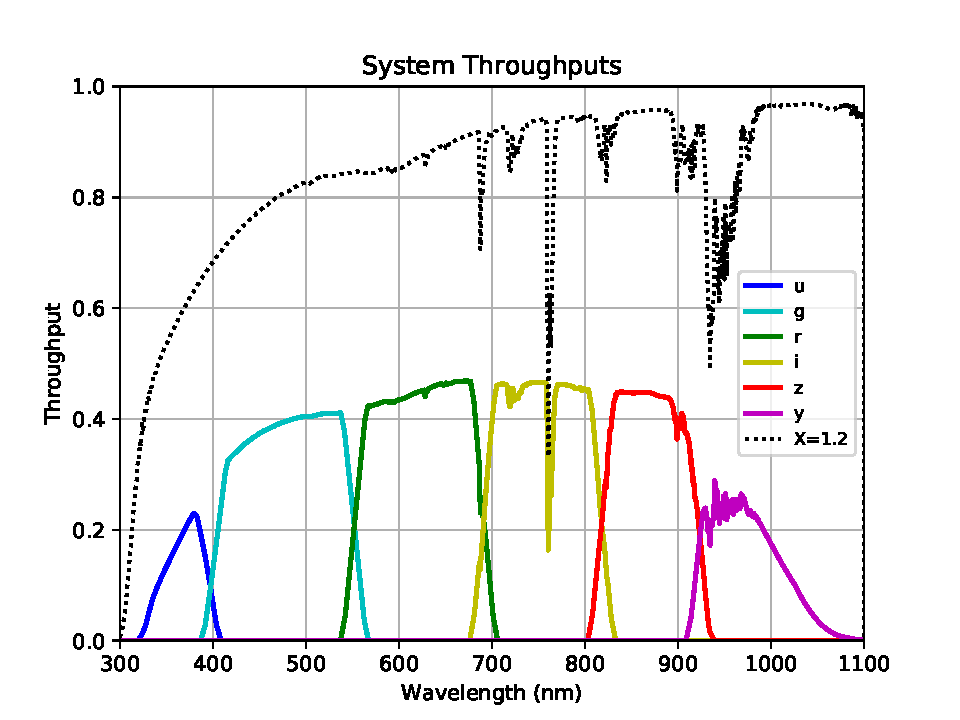
\includegraphics[width=1.1\hsize,clip]{filters_y4.pdf}
\caption{The LSST bandpasses. The vertical axis shows the total throughput. The computation
includes the atmospheric transmission (assuming an airmass of 1.2, % at an altitude of $\sim$56 deg.,
dotted line), optics, and the detector sensitivity.}
\label{Fig:filters}
\end{figure}


The chosen filter complement corresponds to a design ``sweet spot''. We have
investigated the possibility of replacing the $ugrizy$ system with a
filter complement that includes only five filters. For example, each filter
width could be increased by 20\% over the same wavelength range (neither a
shorter wavelength range, nor gaps in the wavelength coverage are desirable
options), but this option is not satisfactory. Placing the red edge of the $u$
band blueward of the Balmer break allows optimal separation of stars and
quasars, and the telluric water absorption feature at 9500\AA\
effectively defines the blue edge of the $y$ band. Of the remaining four
filters ($griz$), the $g$ band is already quite wide. As a last option, the
$riz$ bands could be redesigned as two wider bands. However, this option is also
undesirable because the $r$ and $i$ bands are the primary bands for weak
lensing studies and for star/galaxy separation, and chromatic atmospheric
refraction would worsen the point spread function for a wider bandpass.


\begin{figure}
\hskip -0.12in
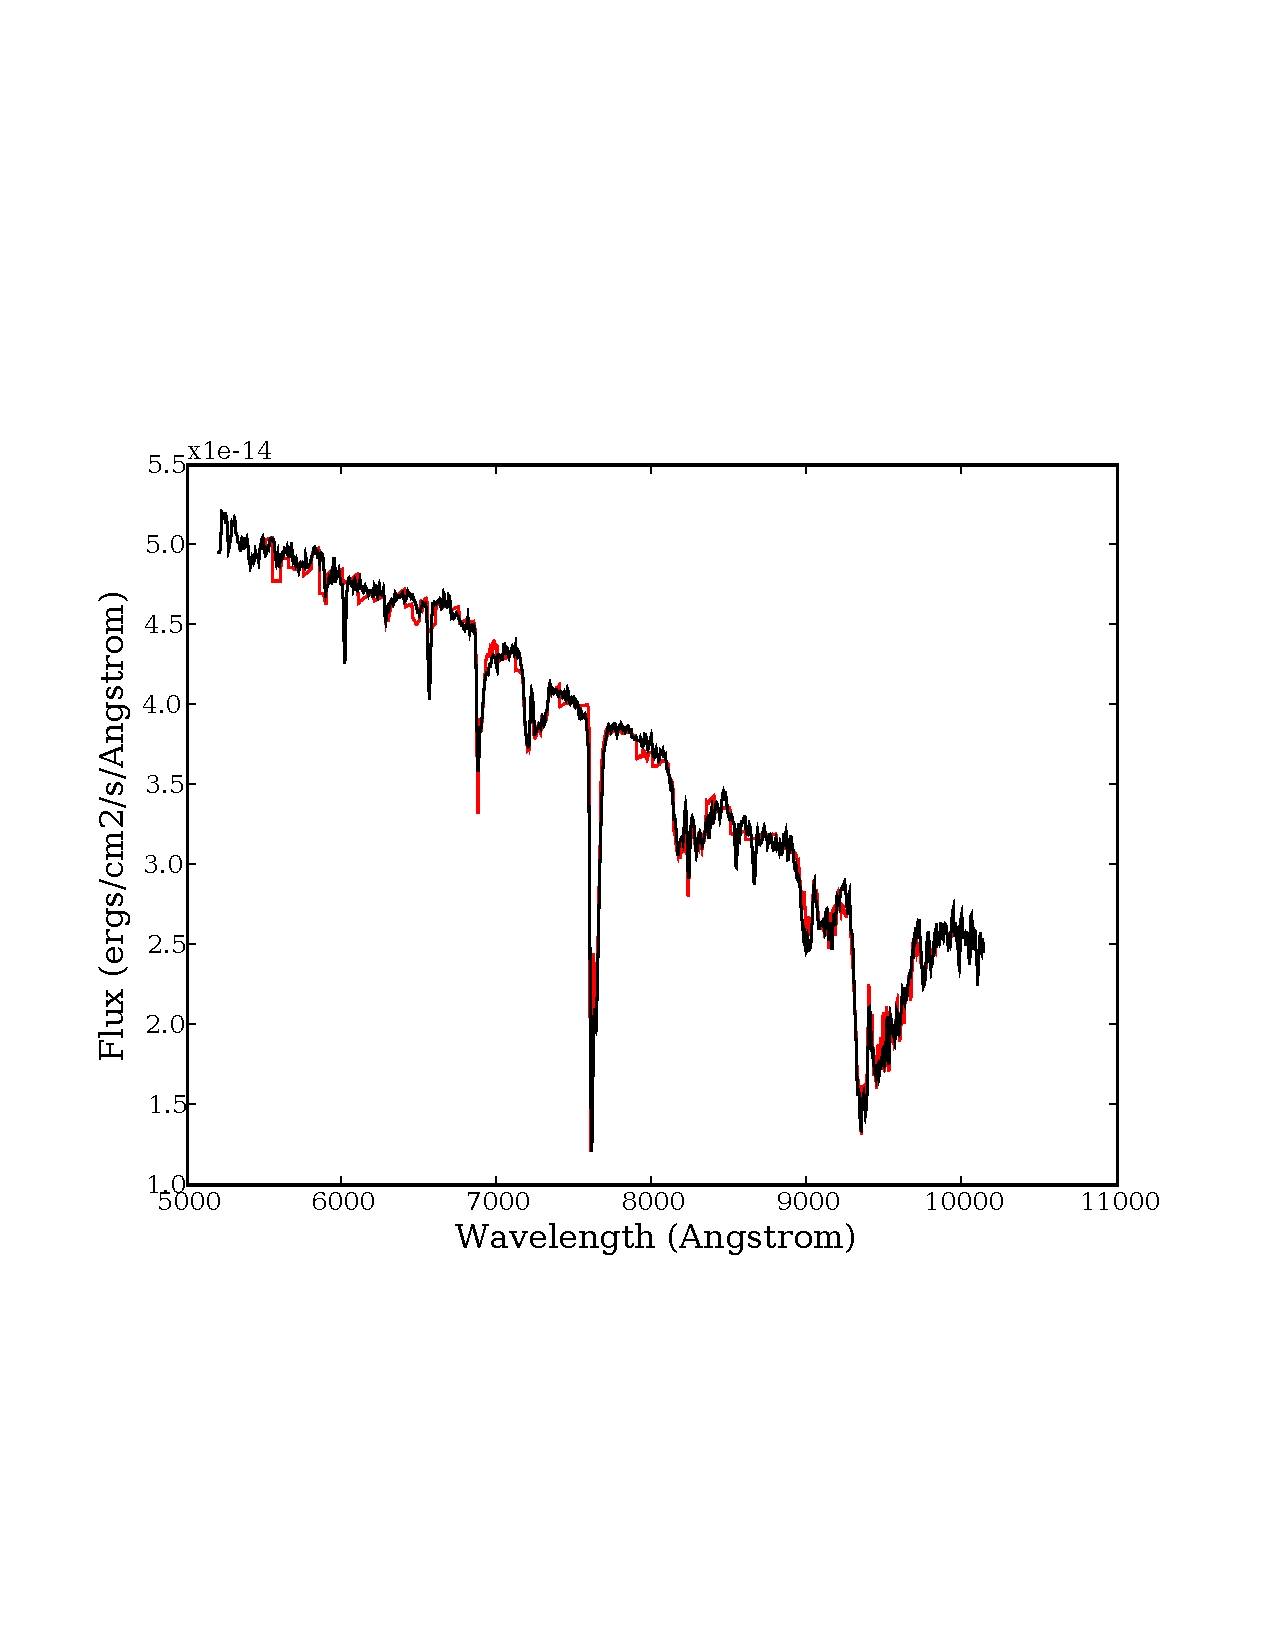
\includegraphics[width=1.1\hsize,clip]{modtran1.pdf}
\caption{An example of determination of the atmospheric opacity by
simultaneously fitting a three-parameter stellar model SED (Kurucz 1979) and
six physical parameters of a sophisticated atmospheric model (MODTRAN, Anderson
et al.~1999) to an observed F-type stellar spectrum ($F_\lambda$). The black
line is the observed spectrum and the red line is the best fit. Note that the
atmospheric water feature around 0.9-1.0 $\mu$m is exquisitely well fit.
The components of the best-fit atmospheric opacity are shown in
Fig.~\ref{Fig:modtran2}. Adapted from Burke et al.~(2007).}
\label{Fig:modtran1}
\end{figure}

\newpage
\subsection{ The Calibration Methods }



\begin{figure}
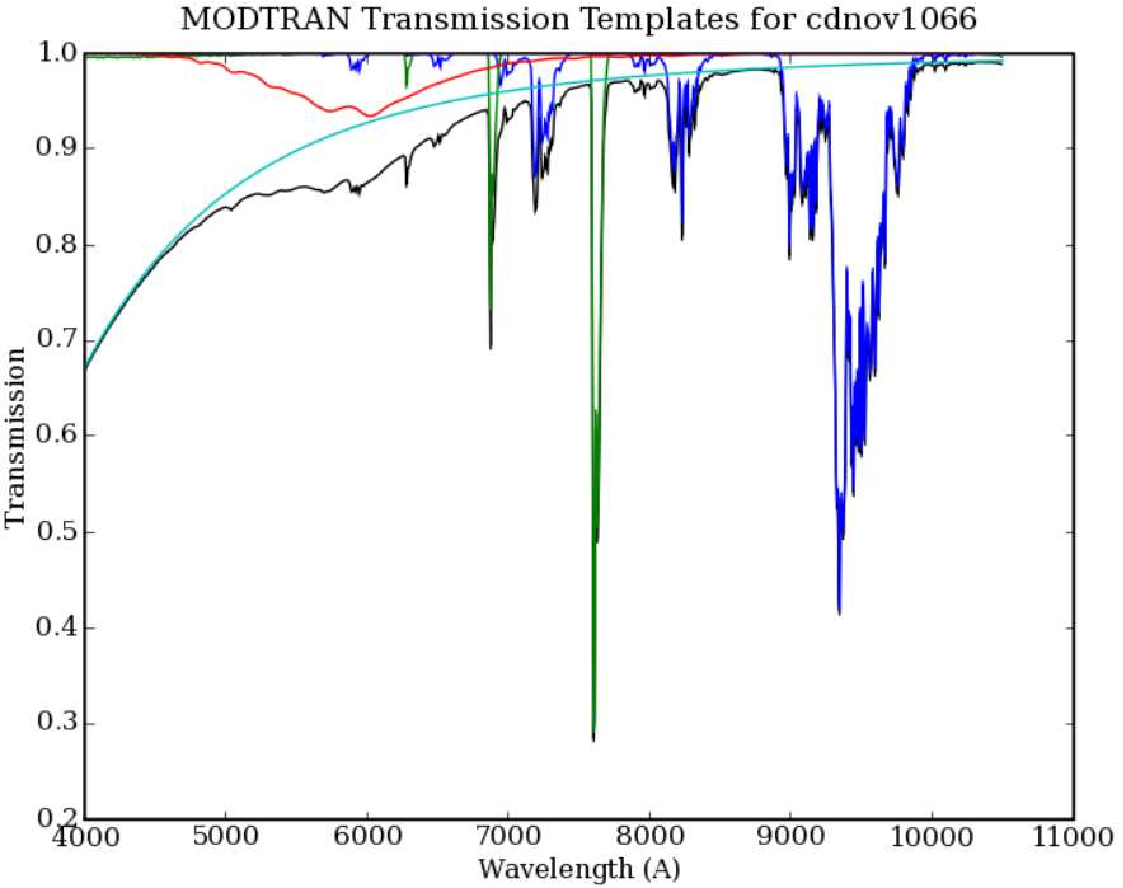
\includegraphics[width=1.0\hsize,clip]{modtran2.pdf}
\caption{The components of the best-fit atmospheric opacity used to
model the observed stellar spectrum shown in Fig.~\ref{Fig:modtran1}.
The atmosphere model (MODTRAN, Anderson et al.~1999) includes six
components: water vapor (blue), oxygen and other trace molecules
(green), ozone (red), Rayleigh scattering (cyan), a gray term
with a transmission of 0.989 (not shown) and an aerosol contribution
proportional to $\lambda^{-1}$ and extinction of 1.3\% at $\lambda$=0.675 \mic\
(not shown). The black line shows all six components combined.
Adapted from Burke et al.~(2007).}
\label{Fig:modtran2}
\end{figure}


Precise determination of the point spread function across each image,
accurate photometric and astrometric calibration, and continuous monitoring
of system performance and observing conditions will be needed to reach the
full potential of the LSST mission. Extensive precursor data including the
SDSS dataset and our own data obtained using telescopes close to
the LSST site of Cerro Pach\'{o}n (e.g., the SOAR and Gemini South telescopes),
as well as telescopes of similar aperture (e.g., Subaru), indicate that the
photometric and astrometric accuracy will be limited not by our instrumentation
or software, but rather by atmospheric effects.
%Active optics will assure superb image quality.

%The required 1\% photometric accuracy is driven by our requirements
%on the photometric redshift accuracy, the separation of stellar populations,
%the ability to detect low-amplitude variable objects, and the search for
%systematic effects in type Ia supernova light curves.

The overall photometric calibration philosophy (Stubbs \& Tonry, 2006) is to measure explicitly, at 1 nm resolution, the
instrumental sensitivity as a function of wavelength using light from a monochromatic source injected
into the telescope pupil. The dose of delivered photons is measured using a calibration photodiode whose quantum
efficiency is known to high accuracy. In addition, the LSST system will explicitly measure the atmospheric transmission
spectrum associated with each image acquired. A
dedicated 1.5-meter auxiliary calibration telescope will obtain spectra of
standard stars in LSST fields, calibrating the atmospheric throughput
as a function of wavelength  (Stubbs et al.~2007;
see Figs.~\ref{Fig:modtran1} and \ref{Fig:modtran2}).
Celestial spectrophotometric sources can be used as a separate means of photometric calibration, albeit only through the
comparison of band-integrated fluxes with synthetic photometry calculations.

This calibration process has been undertaken by the Dark Energy Survey (DES) team, with results reported in Burke et al.~(2017).

SDSS, PS1, and DES data
taken in good photometric conditions have approached the LSST
requirement of 1\% photometric calibration
(Padmanabahn et al.~2008; Schlafly et al.~2012, Burke et al.~2017), although measurements with ground-based telescopes
typically produce data with errors a factor of two or so larger. Analysis of
repeated SDSS scans obtained in varying observing conditions demonstrates that data
obtained in
non-photometric conditions can also be calibrated with
sufficient accuracy (Ivezi\'{c} et al.~2007b), as long as high-quality
photometric data also exist in the region.
The LSST calibration plan builds on this experience gained from the SDSS and other surveys.

The planned calibration process decouples the establishment of a stable and uniform internal
relative calibration from the task of assigning absolute optical flux to
celestial objects.

Celestial sources will be used to refine the internal photometric system and
to monitor stability and uniformity of photometric data. There will be
$>$100 main-sequence stars with $17<r<20$ per detector (14$\times$14 arcmin$^2$)
even at high Galactic latitudes. Standardization of photometric scales will be
achieved through direct observation of stars with well-understood spectral
energy distributions (SEDs), in conjunction with the in-dome calibration system and the atmospheric transmission spectra.

Astrometric calibration will be based on the results from the Gaia mission (Gaia Collaboration 2016), which will provide
numerous high-accuracy astrometric standards in each and every LSST field.

\subsection{     The LSST  Reference Design    }

We briefly describe the reference design for the main LSST system components.
Detailed discussion of the flow-down from science requirements to system
design parameters, and extensive system engineering analysis can be
found in the LSST Science Book (Ch.~2--3).

\begin{figure}
\vskip -0.5in
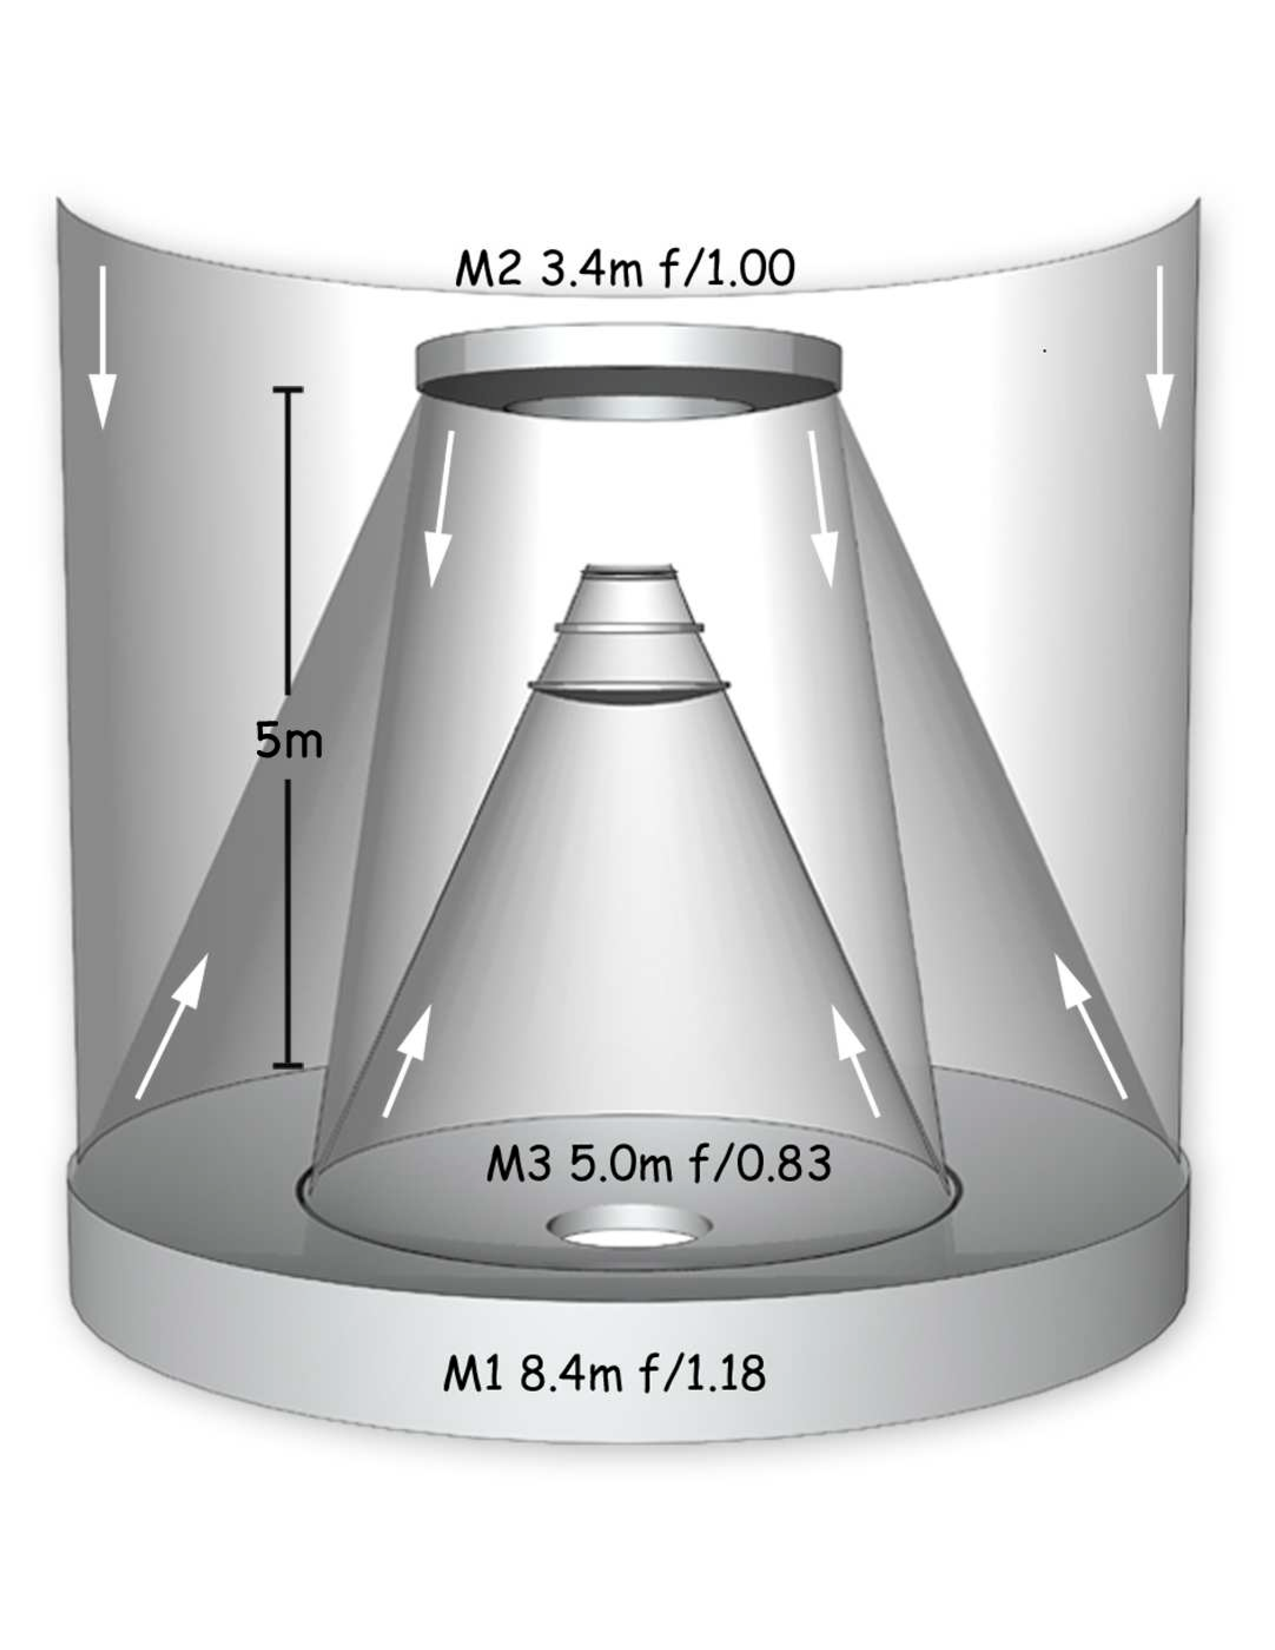
\includegraphics[width=1.0\hsize,clip]{mirrors.pdf}
\vskip -0.5in
\caption{The LSST baseline optical design (modified three-mirror
  Paul-Baker) with its unique
monolithic mirror: the primary and tertiary mirrors are positioned such
that they form a continuous compound surface, allowing them to be polished
from a single substrate.}
\label{Fig:optics}
\end{figure}


\begin{figure}
%\vskip -0.65in
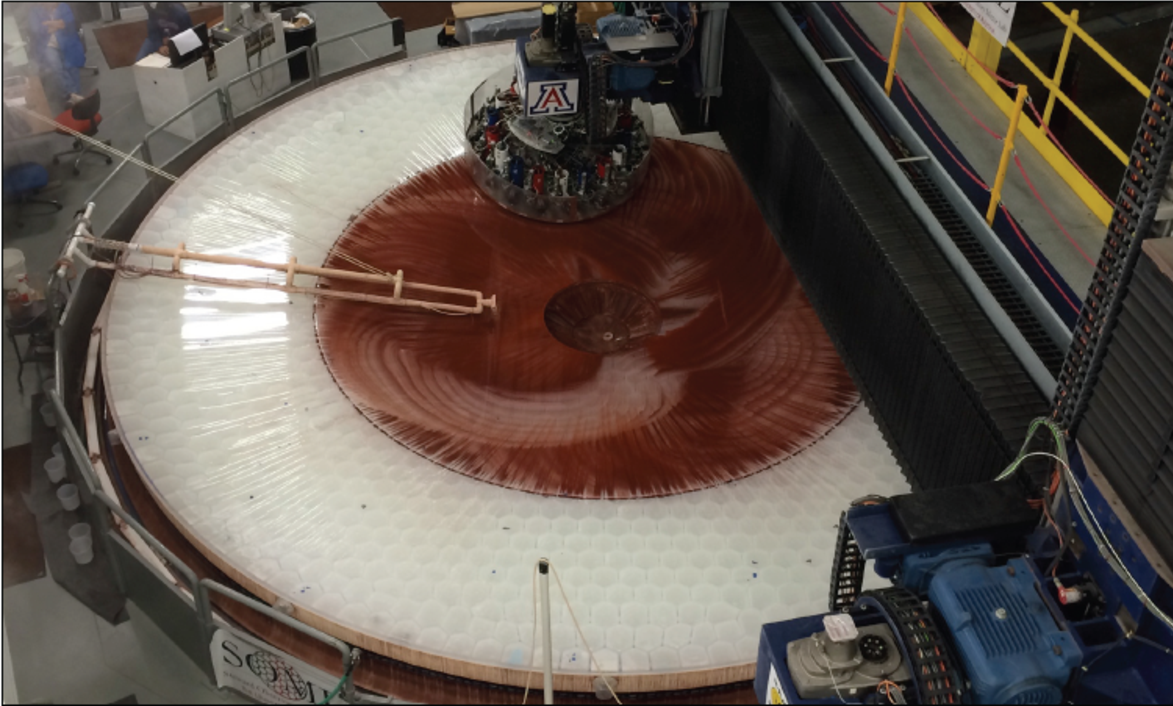
\includegraphics[width=1.0\hsize,clip]{polishing.pdf}
%\vskip -0.65in
\caption{The polishing of the primary-tertiary mirror pair at the Steward Observatory Mirror Lab.}
\label{Fig:polishing}
\end{figure}




\begin{figure}
%\vskip -0.65in
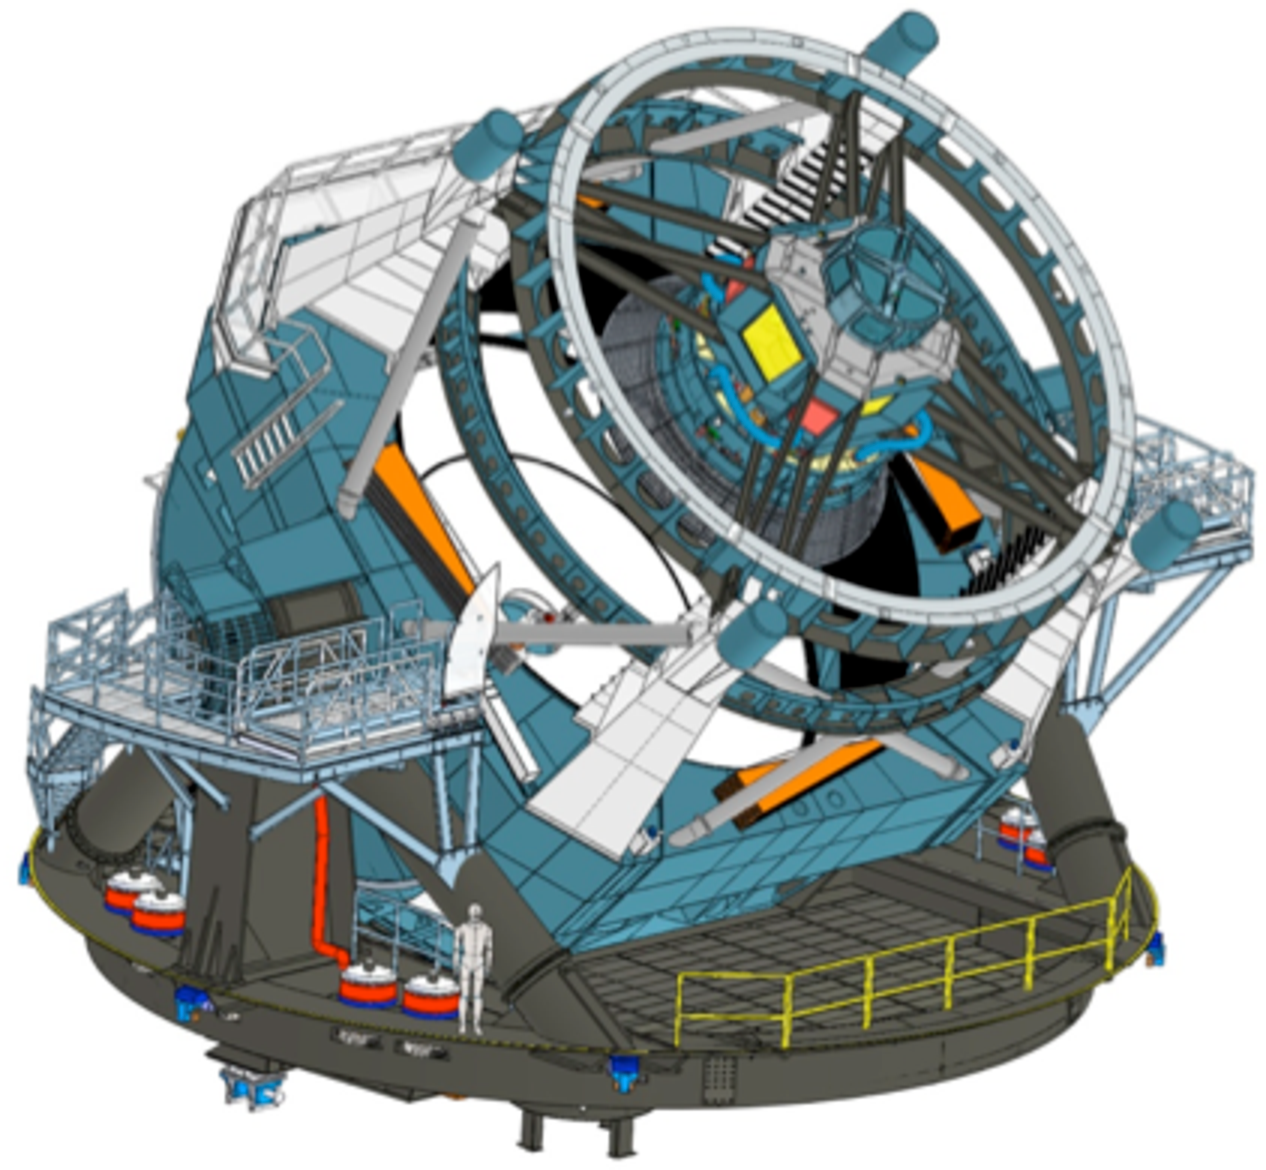
\includegraphics[width=1.0\hsize,clip]{telescopeGreen.pdf}
%\vskip -0.65in
\caption{The baseline design for the
LSST telescope.  The small focal ratio allows for a very squat
telescope, and thus a very stiff structure.  Note the figure of a person for scale.}
\label{Fig:telescope}
\end{figure}




\subsubsection{ Telescope and Site}

The large LSST \'etendue is achieved in a novel three-mirror design (modified
Paul-Baker Mersenne-Schmidt system; Angel, Lesser \& Sarlot 2000) with a very fast $f$/1.234 beam. The optical
design has been optimized to yield a large field of view (9.6 deg$^2$),
with seeing-limited image quality, across a wide wavelength band (320--1050
nm). Incident light is collected by an annular primary mirror, having
an outer diameter of 8.4 m and inner diameter of 5.0 m, creating an effective filled aperture of
$\sim$6.5 m in diameter. The collected light is reflected to a 3.4 m convex secondary, then onto
a 5 m concave tertiary, and finally  into the three refractive lenses of the camera (see Fig.~\ref{Fig:optics}).
In broad terms, the primary-secondary mirror pair acts as a beam condenser, while the aspheric portion of
the secondary and tertiary mirror acts as a Schmidt camera.  The 3-element refractive optics of the camera
correct for the chromatic aberrations induced by the necessity of a thick dewar window and flatten the
focal surface.  During design optimization, the primary and tertiary mirror surfaces were placed such that the primary's
inner diameter coincides with the tertiary's outer diameter, thus making it possible to fabricate the mirror pair from a
single monolithic blank using spin-cast borosilicate technology. The secondary mirror is fabricated from
a thin 100 mm thick meniscus substrate, made from Corning's ultra-low expansion material. All
three mirrors will be actively supported to control wavefront distortions
introduced by gravity and environmental stresses on the telescope.
The primary-tertiary mirror and the secondary mirror were
cast\footnote{http://www.lsst.org/News/enews/m1m3-1004.html}  in 2008
and 2009.  The primary-tertiary mirror pair is currently being polished at the Steward Observatory Mirror Lab
(see Fig.~\ref{Fig:polishing}) and is expected to be completed in the second half of 2014.  The polishing of
the secondary should start around that time.


\begin{figure}
%\vskip -1.3in
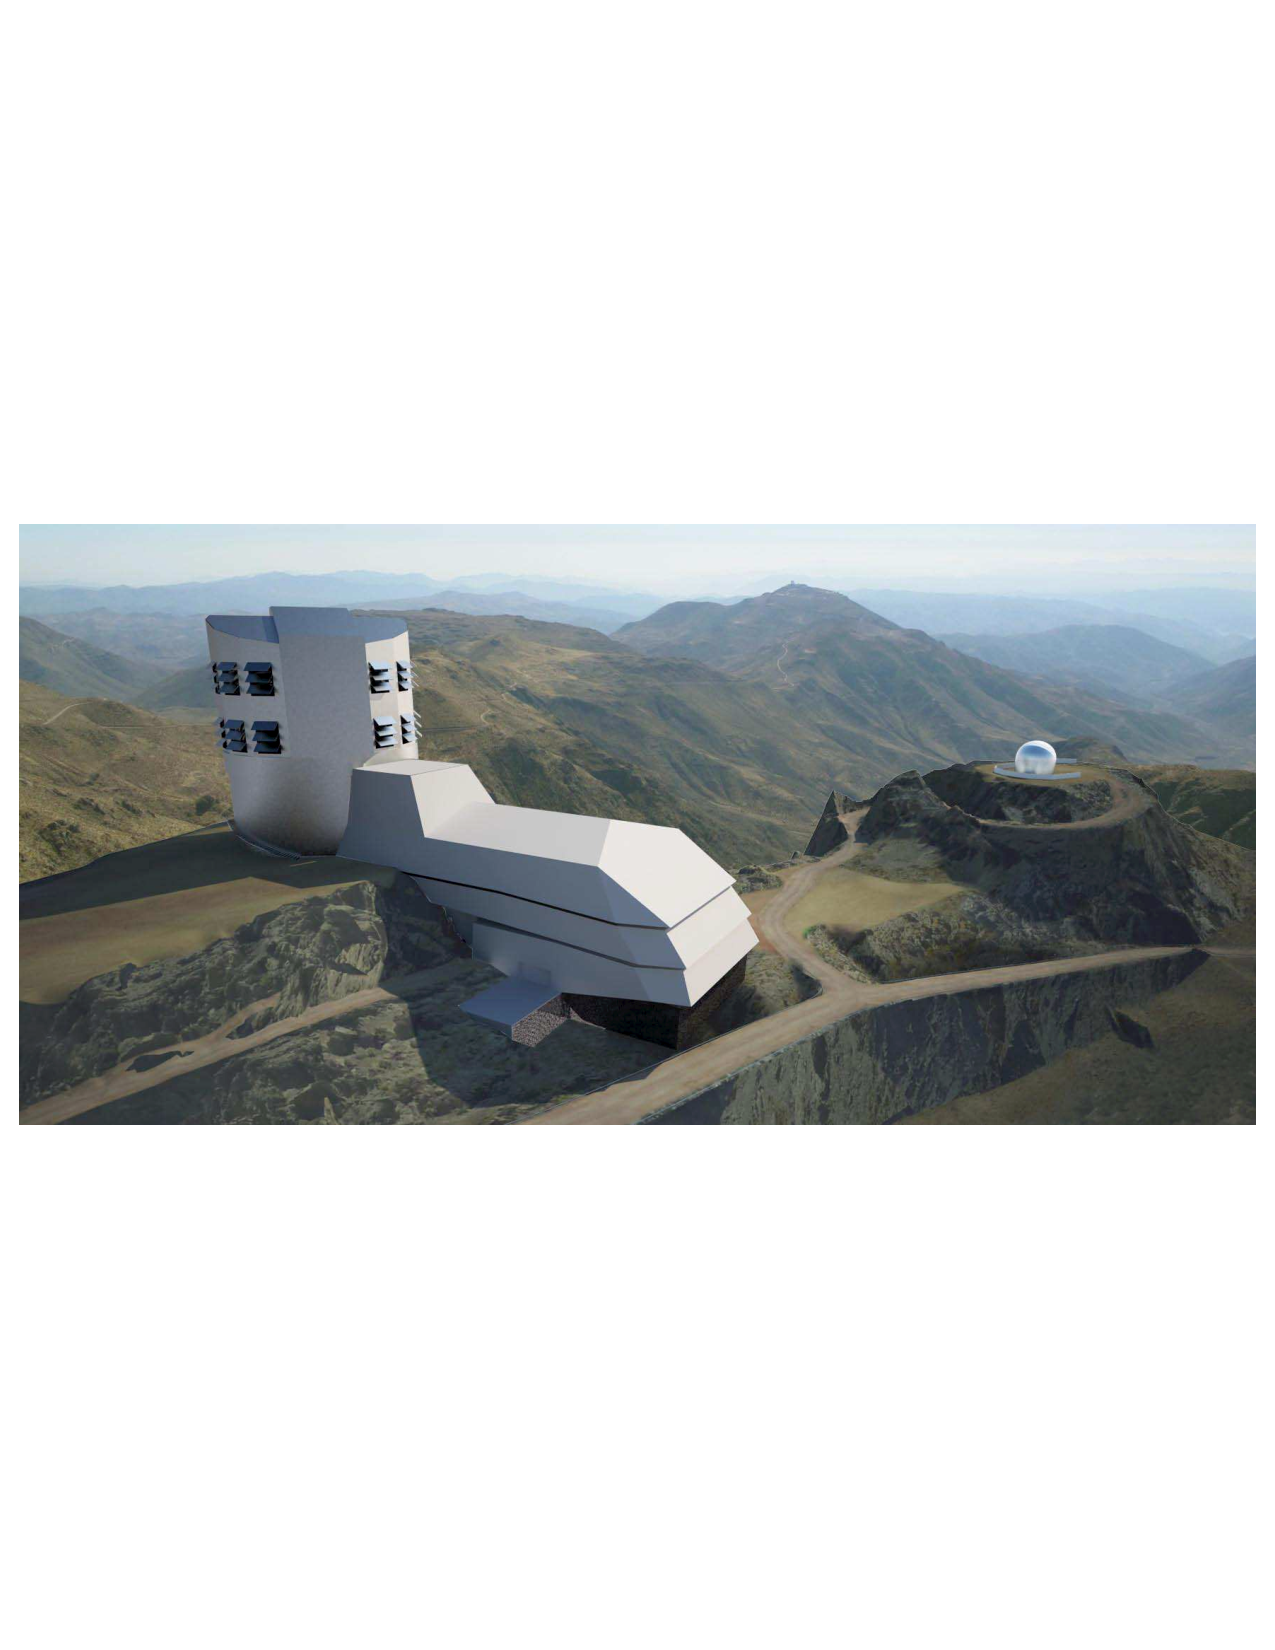
\includegraphics[width=1.0\hsize,clip]{observatoryFull.pdf}
%\vskip -1.4in
\caption{The LSST Observatory: artist's rendering of the dome enclosure
with the attached summit support building on Cerro Pach\'{o}n. The LSST calibration
telescope is shown on an adjacent rise to the right.}
\label{Fig:observatory}
\end{figure}

The LSST Observing Facility (Fig.~\ref{Fig:observatory}),
consisting of the telescope enclosure and summit support building, will be constructed atop Cerro Pach\'{o}n in northern Chile,
sharing the ridge with the Gemini South and SOAR telescopes\footnote{Coordinates listed in older versions
of this paper were incorrect. We thank E. Mamajek for pointing this error to us.}
% old, WRONG: (latitude: S 30$^\circ$ 10$'$ 20.1$"$; longitude: W 70$^\circ$ 48$'$ 0.1$"$; elevation: 2123 m;
% NEW: from Mamajek (2012, arXiv:1210.1616, Table 3, GPS values):
(latitude: S 30$^\circ$ 14$\arcmin$ 40.68$\arcsec$; longitude: W 70$^\circ$ 44$\arcmin$ 57.90$\arcsec$; elevation: 2652 m;
Mamajek 2012).  The telescope enclosure houses a compact, stiff
telescope structure (see Fig.~\ref{Fig:telescope}) atop a 15 m high concrete pier
with a fundamental frequency of 8 Hz, that is crucial for achieving the required fast slew-and-settle times.  The height of the pier was set to place the telescope above the degrading
effects of the turbulent ground layer.  Capping the telescope
enclosure is a 30 m diameter dome with extensive ventilation to reduce
dome seeing
%(local air turbulence that can distort images)
and to maintain a uniform thermal environment over the course of the night.  Furthermore, the summit support
building has been oriented with respect to the prevailing winds to shed its turbulence away from the
telescope enclosure.  The summit support building includes a coating chamber for recoating the three LSST mirrors and
clean room facilities for maintaining and servicing the camera.




\vskip 0.2in
\subsubsection{ Camera }


The LSST camera provides a 3.2 Gigapixel flat focal plane array, tiled by 189
4K$\times$4K CCD science sensors with 10 $\mu$m pixels (see Figs.~\ref{Fig:camera}
and \ref{Fig:fov}). This pixel count is a direct consequence of sampling the
9.6 deg$^2$ field-of-view (0.64m diameter) with 0.2$\times$0.2 arcsec$^2$
pixels (Nyquist sampling in the best expected seeing of $\sim$0.4 arcsec).
The sensors are deep depleted high resistivity silicon back-illuminated devices with
a highly segmented architecture that enables the entire array to be read in 2 seconds.
The detectors are grouped into 3$\times$3 rafts (see Fig.~\ref{Fig:raft}); each
contains its own dedicated electronics. The rafts are mounted on a silicon carbide
grid inside a vacuum cryostat, with an intricate thermal control system that maintains
the CCDs at an operating temperature of 173 K. The entrance window to the
cryostat is the third (L3) of the three refractive lenses in the camera. The other
two lenses (L1 and L2) are mounted in an optics structure at the front of the camera
body, which also contains a mechanical shutter, and a carousel assembly that holds
five large optical filters. The sixth optical filter can
replace any of the five via a procedure accomplished during daylight hours.



\begin{figure}[t!]
%\hskip -1.7in
%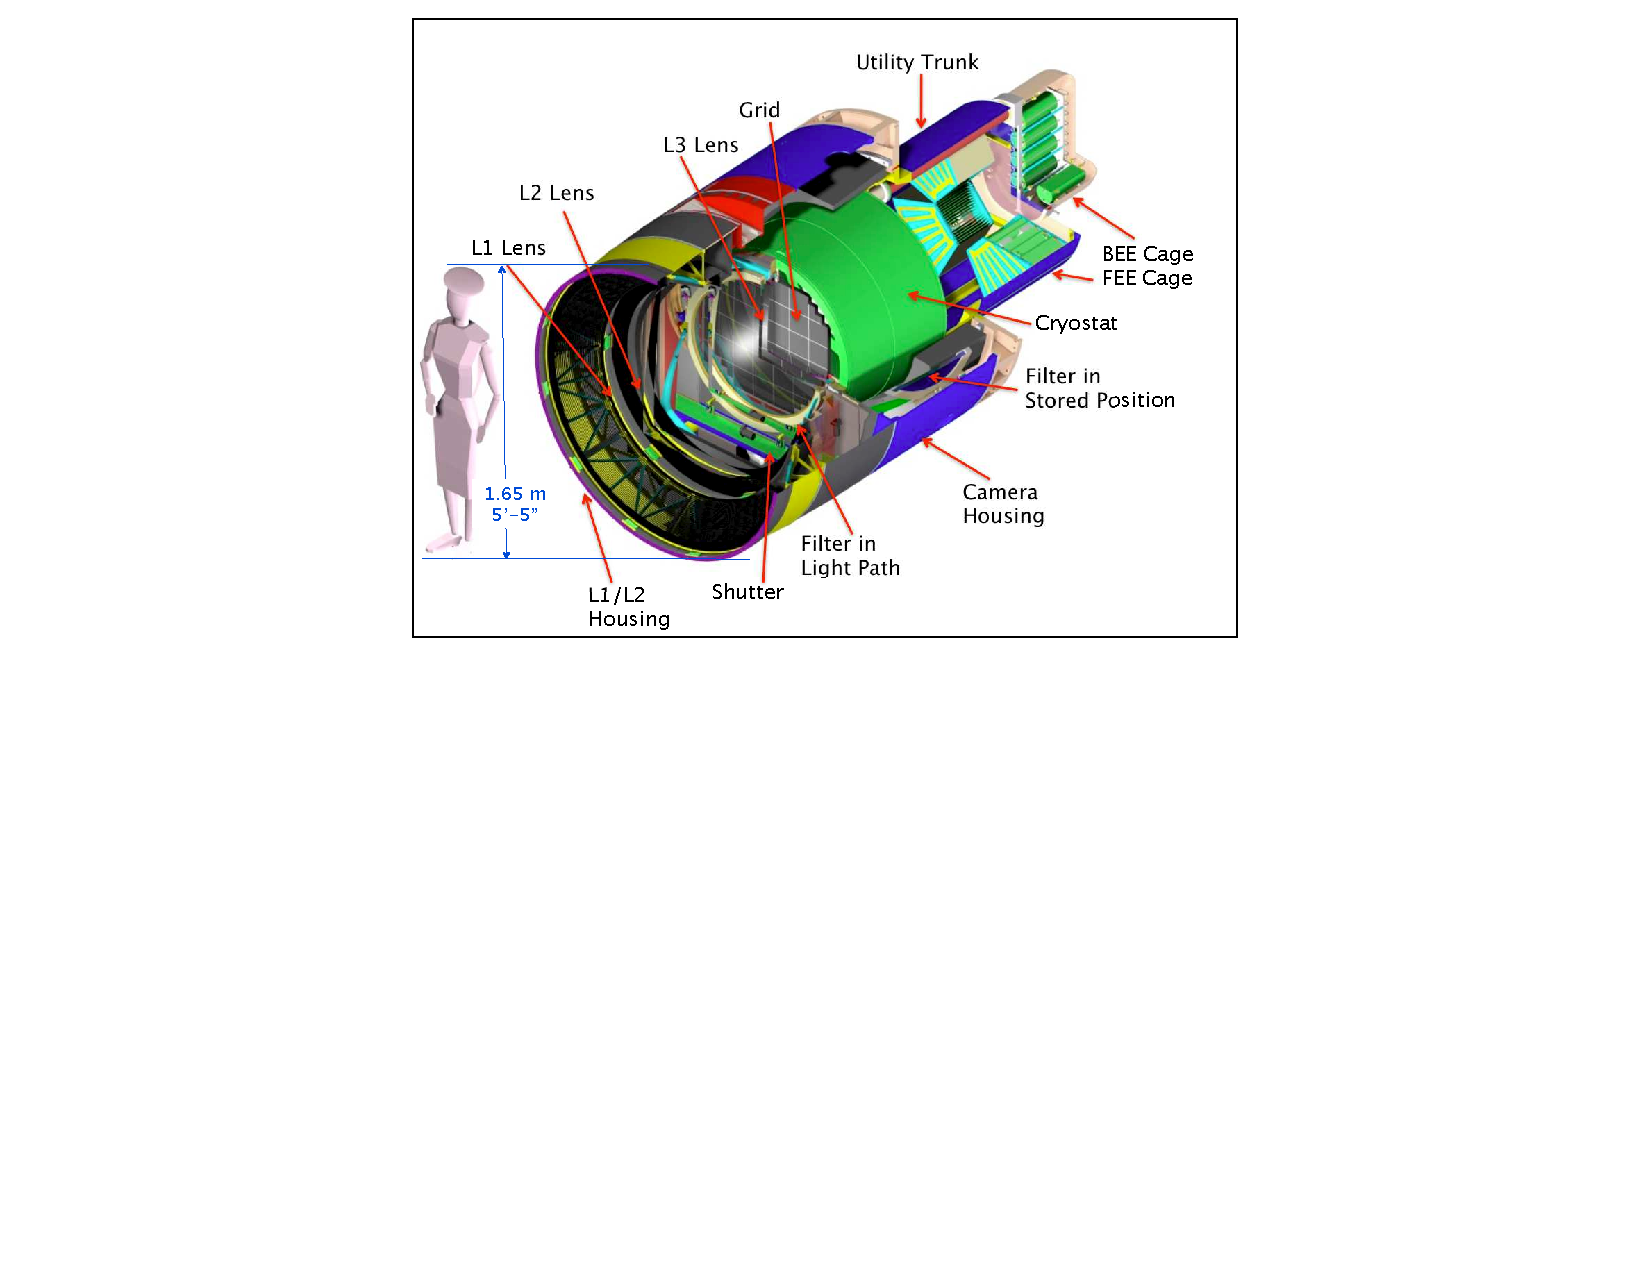
\includegraphics[width=1.55\hsize,angle=90.0,clip]{camera2009.pdf}
%\vskip -2.5in
%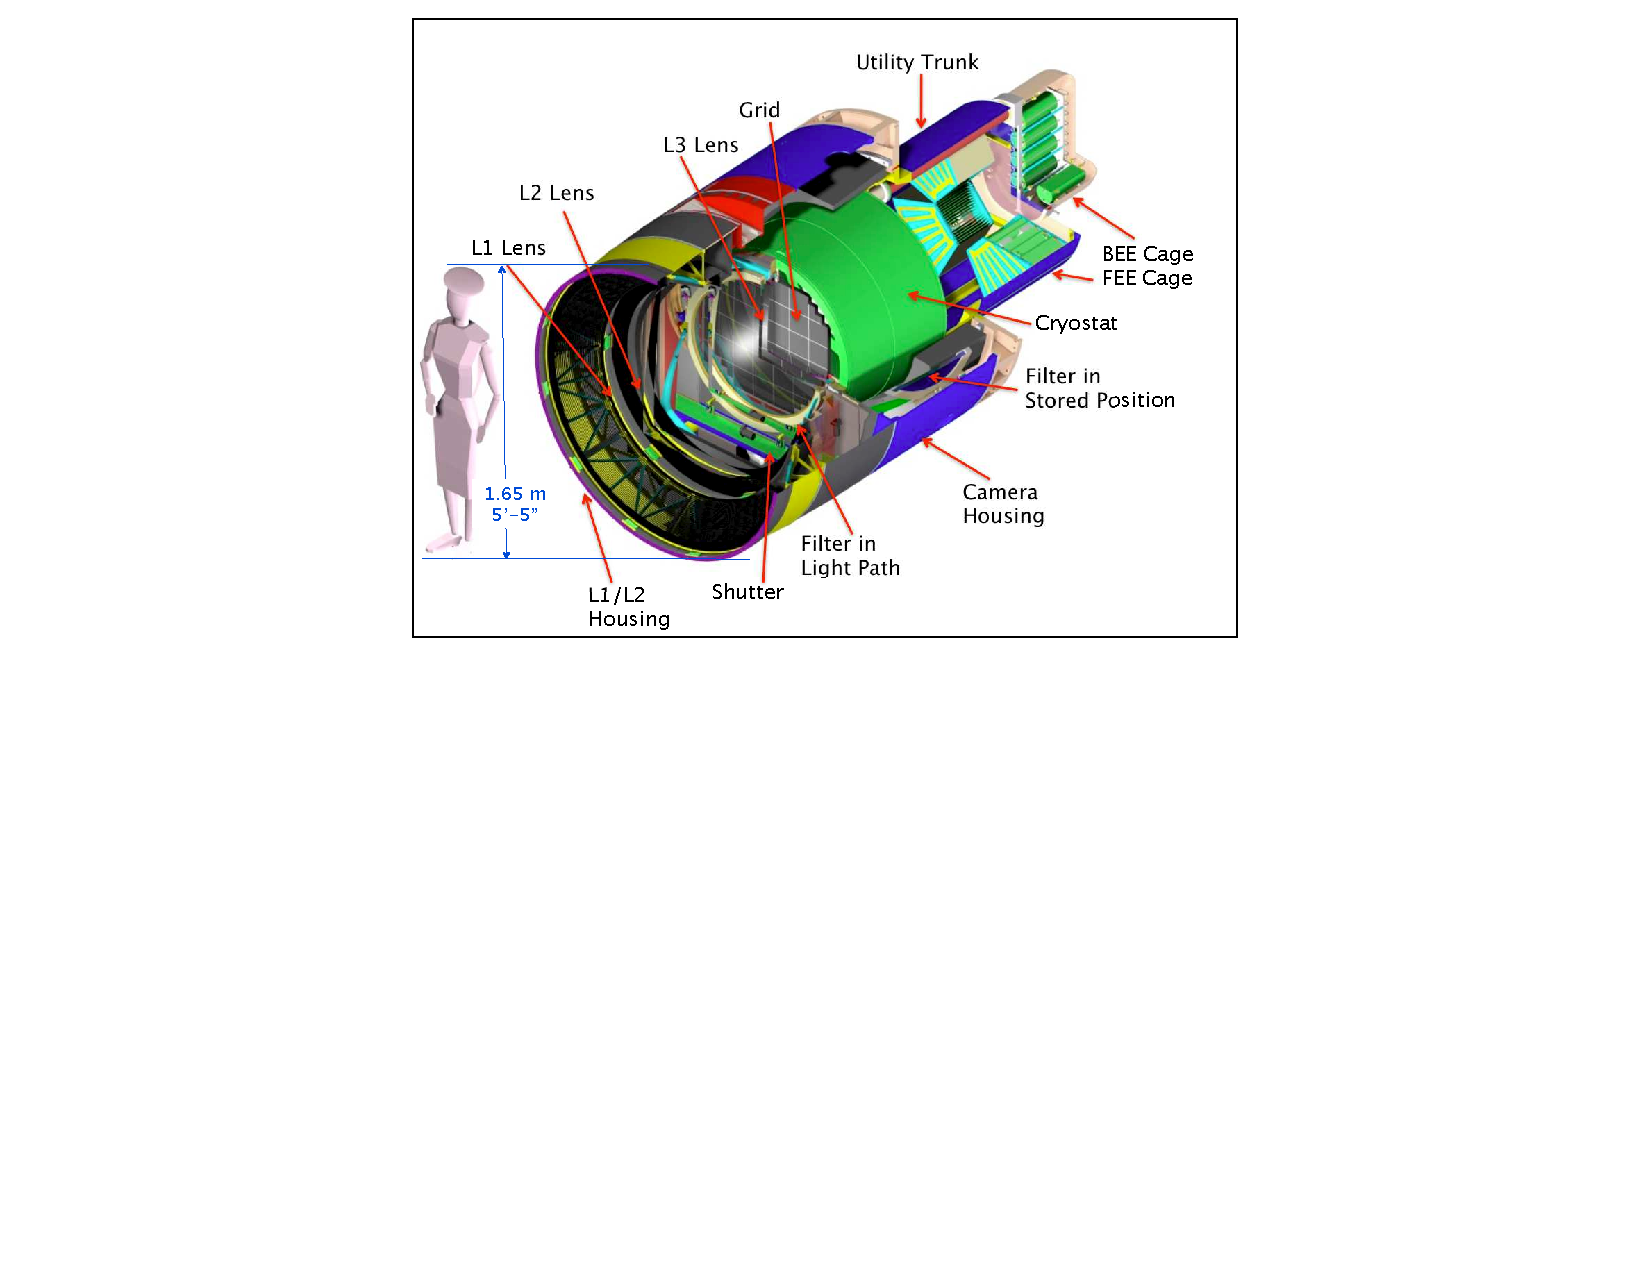
\includegraphics[width=1.55\hsize,angle=90.0,clip]{camera2009.pdf}
\hskip 0.1in
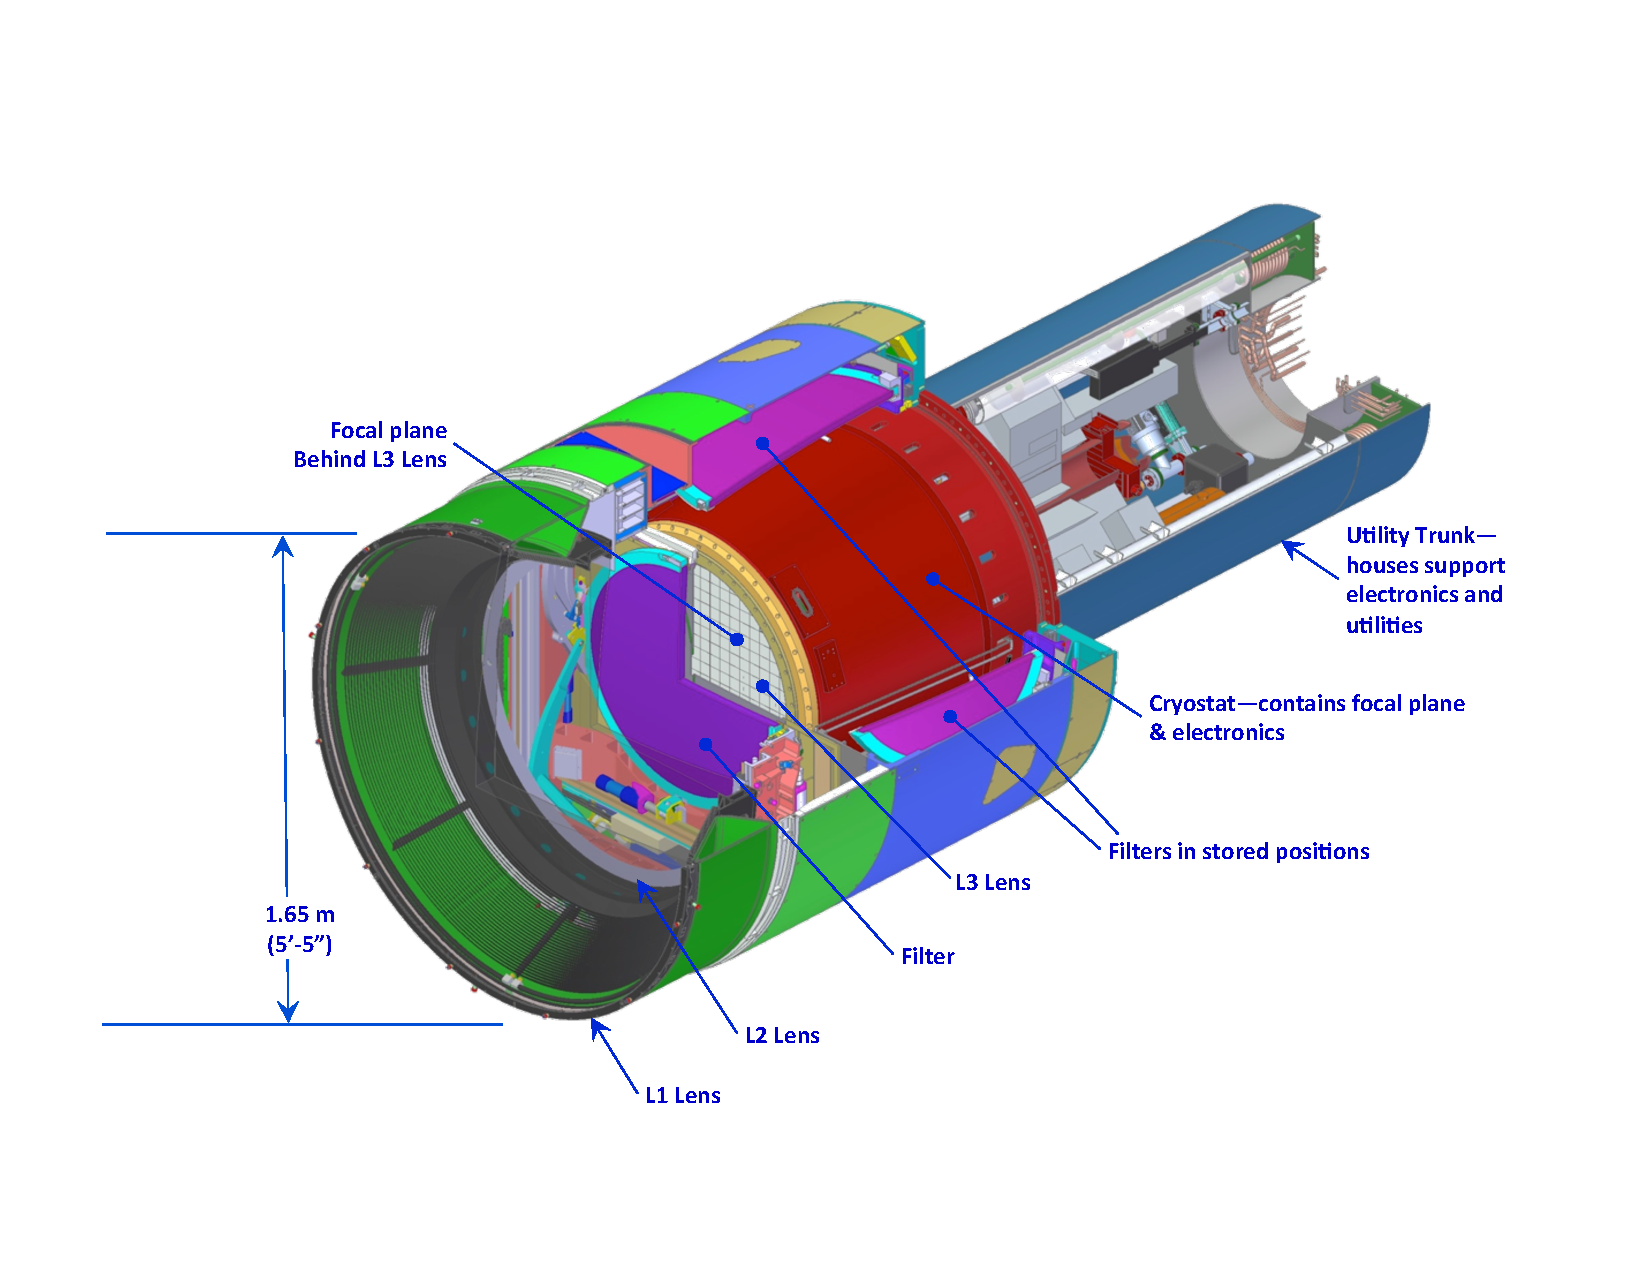
\includegraphics[width=0.45\textwidth]{CameraFigureUpdated.pdf}
\caption{A cutaway view of LSST camera. The camera is positioned in the middle of the telescope.  The shutter (not shown) is positioned between the filter and lens L3.}
\label{Fig:camera}
\end{figure}


\begin{figure}[ht]
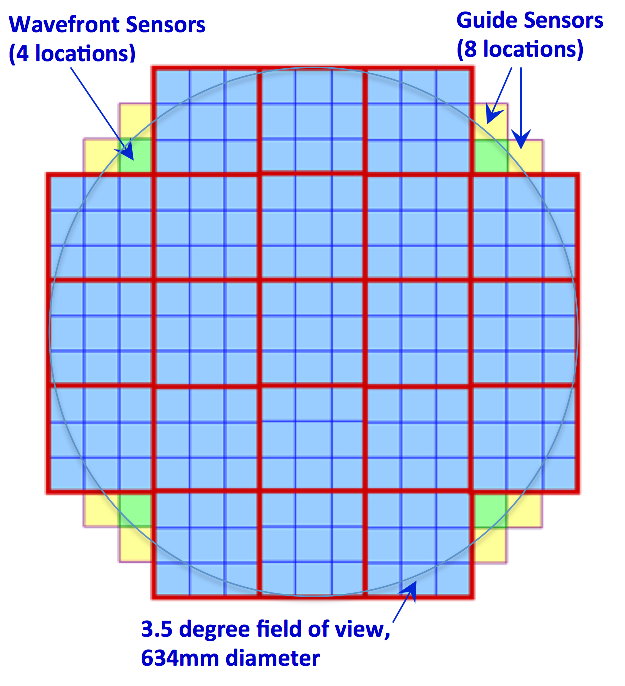
\includegraphics[width=1.0\hsize,clip]{fov-updated-cropped.pdf}
\caption{The LSST focal plane. Each cyan square represents one
$4096\times4096$ pixel sensor. Nine sensors are assembled into a
raft; the 21 rafts are outlined in red. There are 189 science sensors, each
with 16.8 megapixels, for a total of 3.2 gigapixels.}
\label{Fig:fov}
\end{figure}

\begin{figure}[ht]
%\hskip -1.6in
%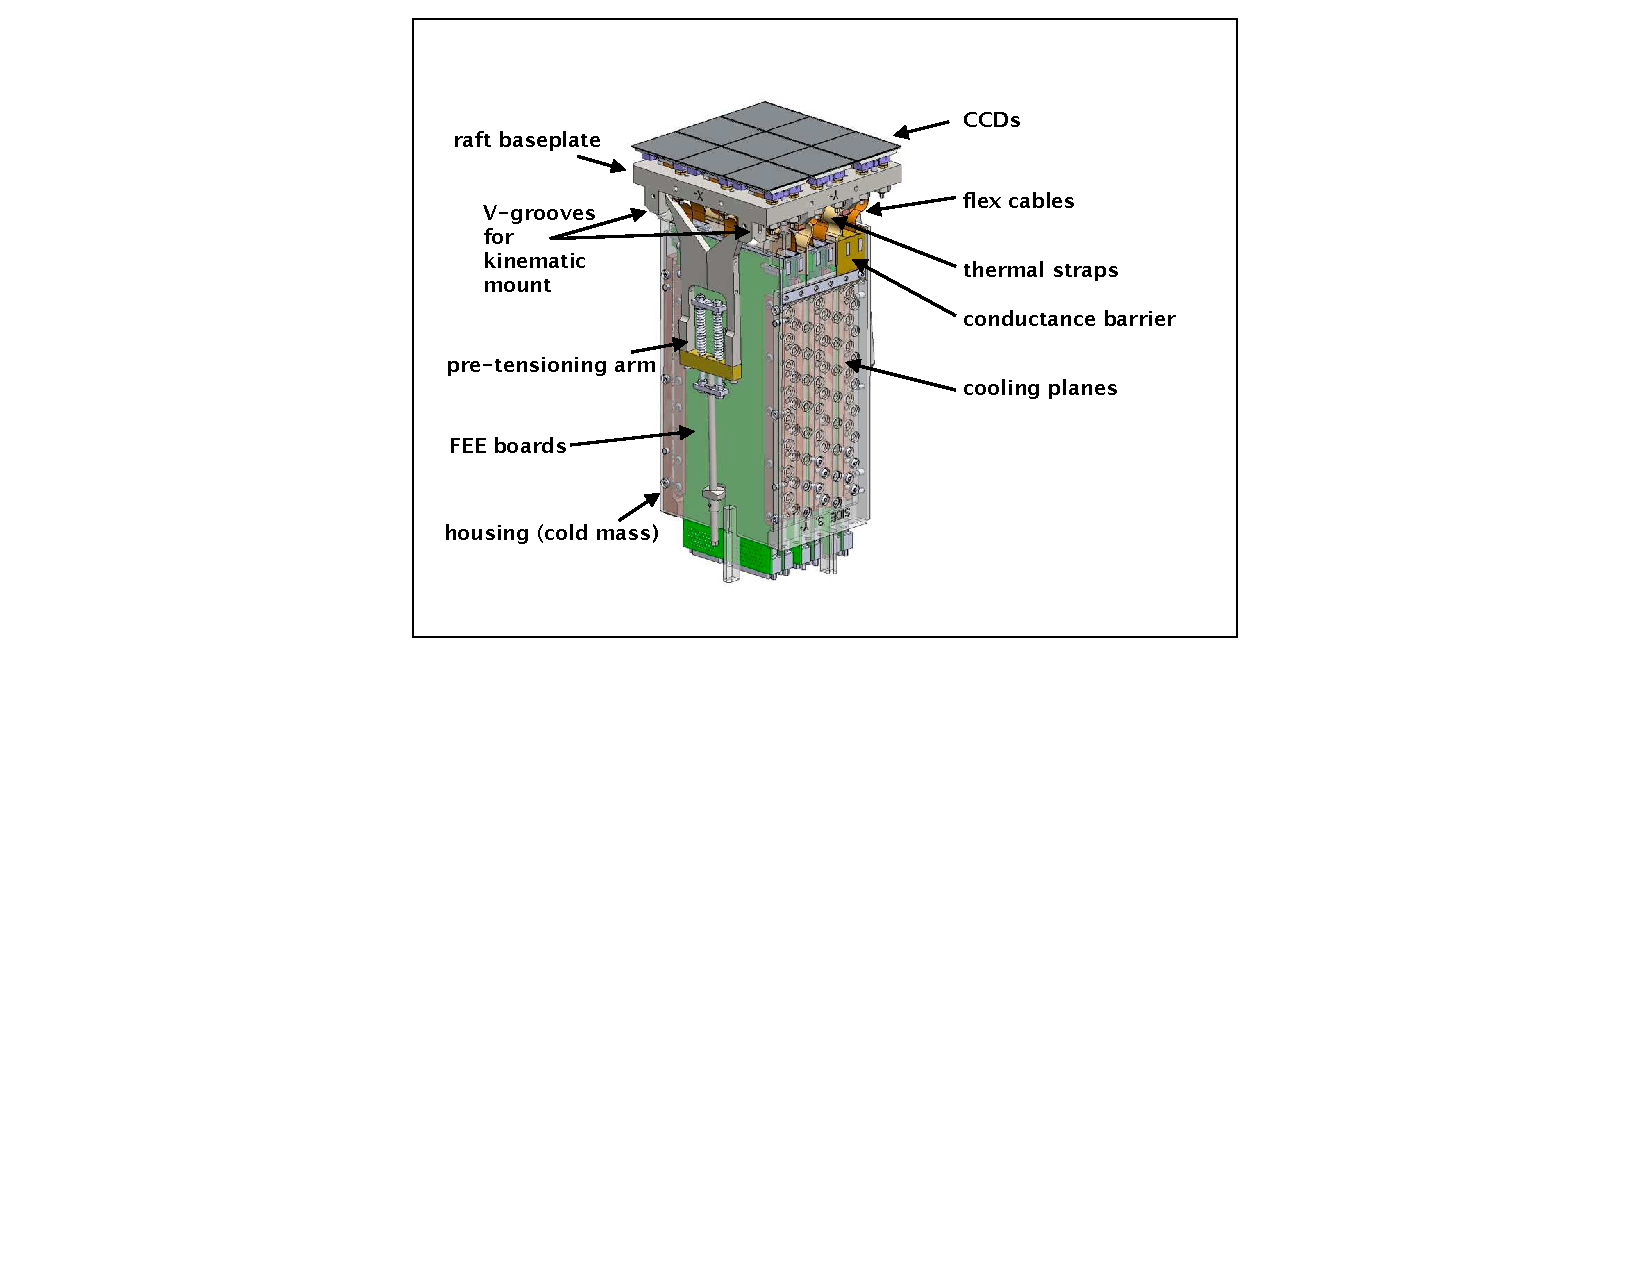
\includegraphics[width=1.5\hsize,angle=90.0,clip]{raft.pdf}
%\vskip -2.5in
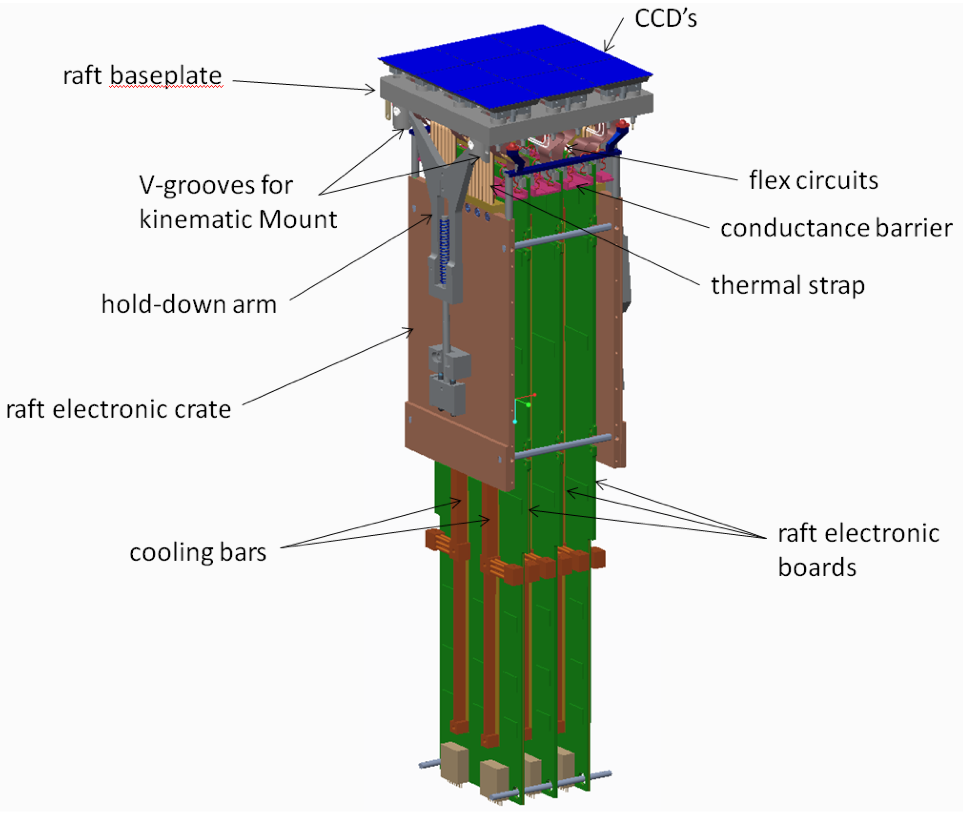
\includegraphics[width=1.\hsize,clip]{raft-updated-cropped.pdf}
\caption{The LSST raft module with integrated front-end electronics
and thermal connections. Each raft (corresponding to the red squares
in Fig.~\ref{Fig:fov})
includes 9 sensors, and can be replaced.}
\label{Fig:raft}
\end{figure}



\vskip 0.2in
\subsubsection{ Data Management }
\label{sec:dm}

The rapid cadence and scale of the LSST observing program will produce
approximately 15 TB per night of raw imaging data\footnote{For
  comparison, the volume of all imaging data collected over a decade
  and published in SDSS Data Release 7 (Abazajian et al.~2009) is approximately 16 TB.}. The large data volume, the real-time aspects, and the complexity of processing involved makes it impractical to defer the data reduction to the LSST end-users. Instead, the data collected by the LSST system will be automatically reduced to scientifically useful catalogs and images by the LSST Data Management (DM) system.
\\

The principal functions of the LSST Data Management system are to:
\begin{itemize}
\item Process, in real time, the incoming stream of images generated by the camera system during observing by archiving raw images, generating alerts to new sources or sources whose properties have changed, and updating the relevant catalogs (``Level 1'' data products; \S~\ref{Sec:dp}).
\item Periodically process the accumulated survey data to provide a
  uniform photometric and astrometric calibration, measure the
  properties of all detected objects, and characterize objects based on their time-dependent behavior. The results of such a processing run form a {\em Data Release} (DR), which is a static, self-consistent data set suitable for use in performing scientific analyses of LSST data and publication of the results (the ``Level 2'' data products; \S~\ref{Sec:dp}). All data releases will be archived for the entire operational life of the LSST archive.
\item Facilitate the creation of added-value (``Level 3'';
  \S~\ref{Sec:dp}) data products, by providing suitable software,
  application programming interfaces (APIs),
and computing infrastructure at the LSST data access centers.
\item Make all LSST data available through an interface that utilizes
community-based standards   to the maximum possible extent. Provide
  enough processing, storage, and network bandwidth to enable user
  analyses of the data without the need for petabyte-scale data
  transfers.
\end{itemize}

Over the ten years of LSST operations and 11 data releases, this processing will result in a cumulative {\em processed} data size
approaching 500 petabytes (PB) for imaging, and over 50 PB for the
catalog databases. The final data release catalog database alone is expected
to be approximately 15 PB in size.
\\

\begin{figure}
%
% NOTE NOTE NOTE: The source of this figure is in DMsandwich.pptx.
% Edit that file and save it as PDF when an update is needed.
%
\hskip -0.2in
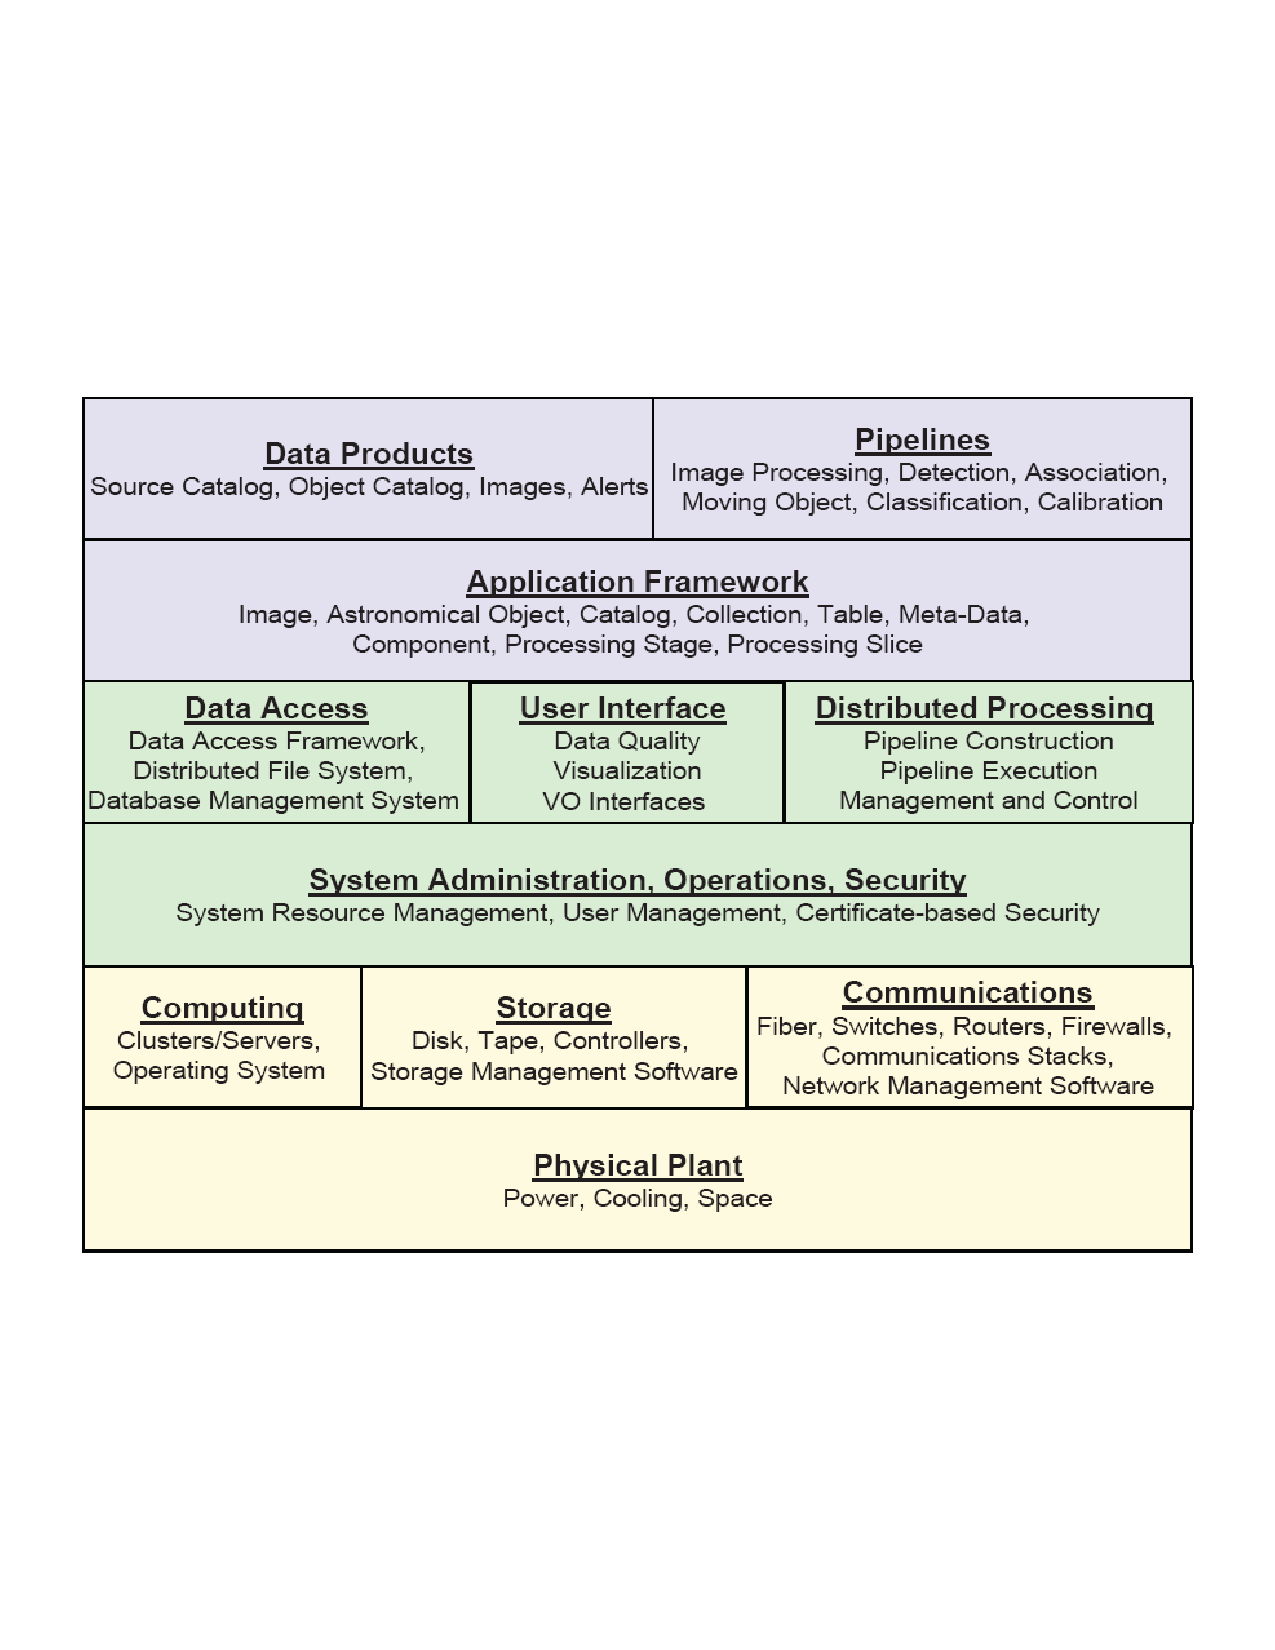
\includegraphics[width=1.1\hsize,clip]{DMsandwich.pdf}
\caption{The three-layered architecture of the data management system
(application [red, top], middleware [purple, middle], and infrastructure [blue, bottom] layers) enables scalability, reliability, and evolutionary capability.}
\label{Fig:DM1}
\end{figure}

The data management system is conceptually divided into three layers: an
infrastructure layer consisting of the computing, storage, and
networking hardware and system software; a middleware layer, which
handles distributed processing, data access, user interface, and
system operations services; and an applications layer, which includes
the data pipelines and products and the science data archives (see
Fig.~\ref{Fig:DM1}).

\begin{figure*}
%
% NOTE NOTE NOTE: The source of this figure is in DMX2.pptx
% Edit that file and save it as PDF when an update is needed.
%
\hskip 0.25in
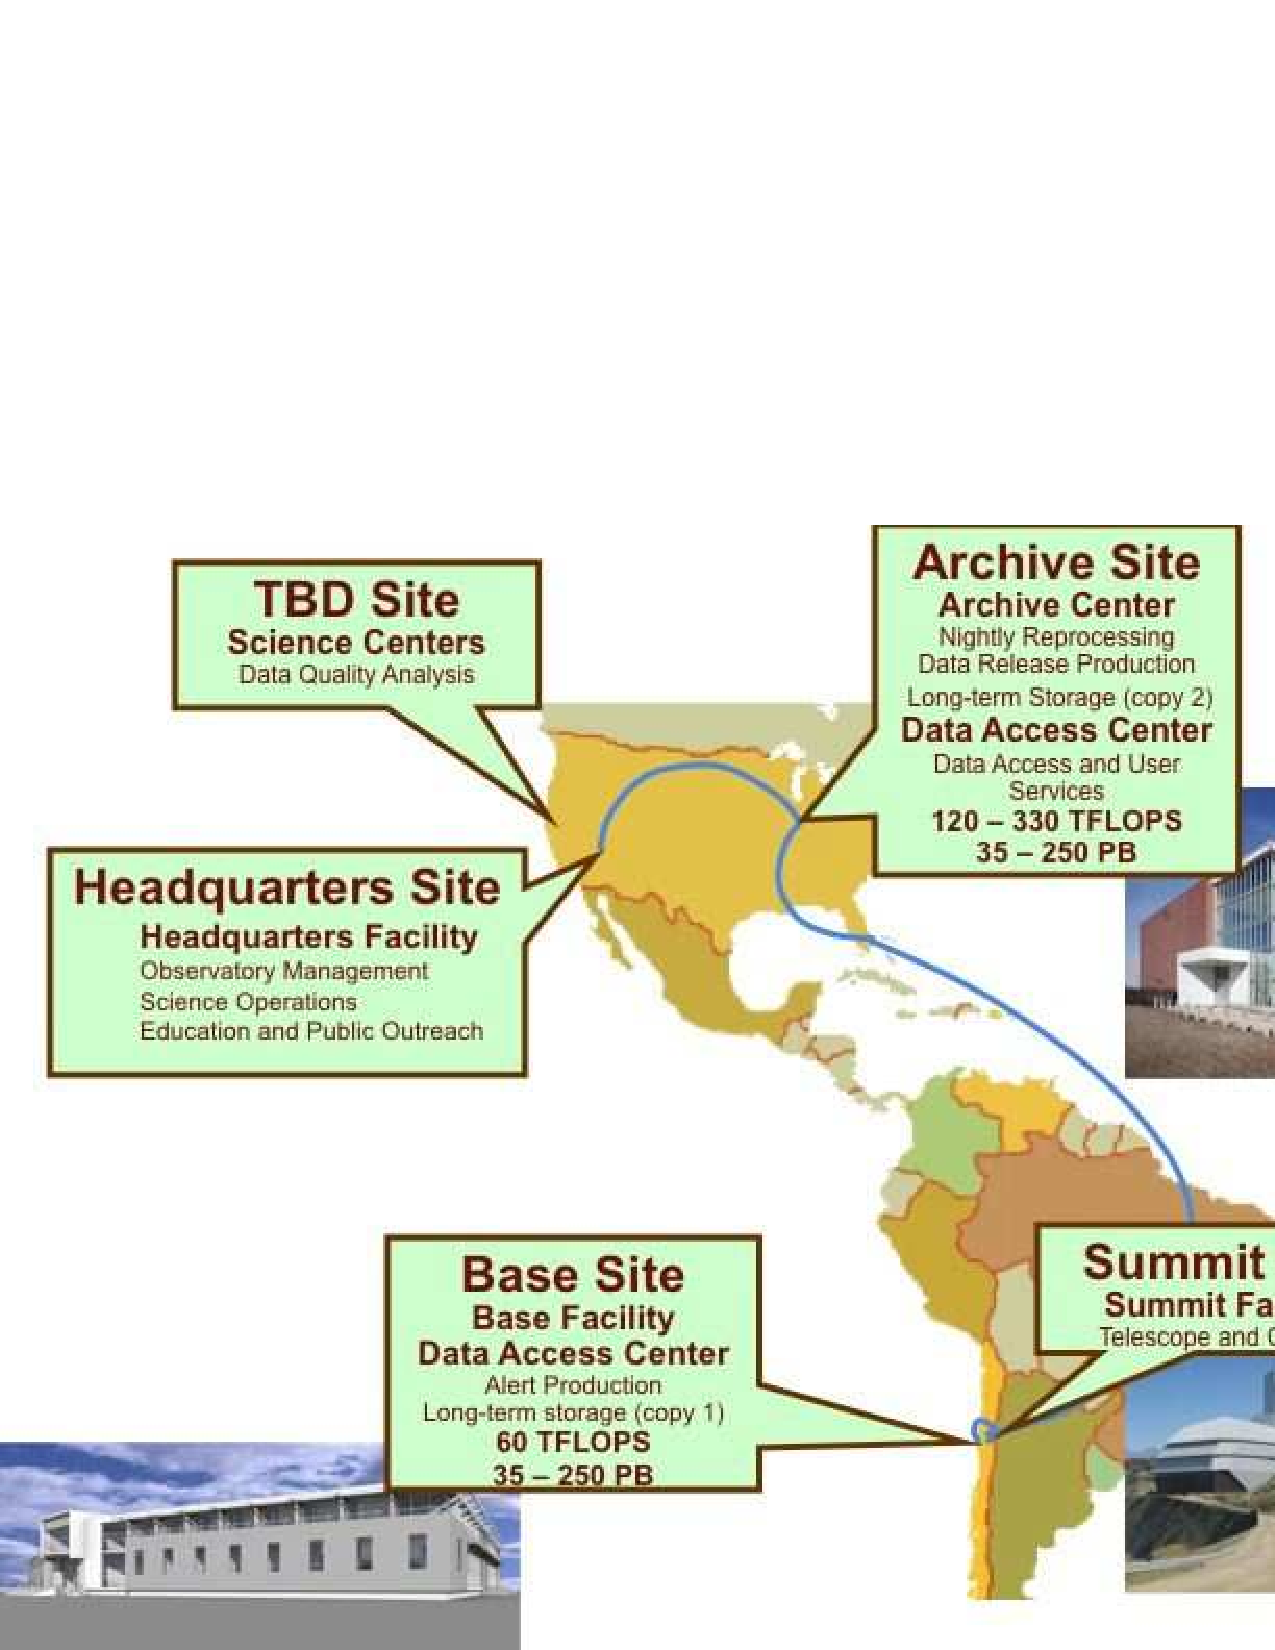
\includegraphics[width=0.95\hsize,clip]{DMX2.pdf}
\caption{The LSST data flow from the mountain summit/base facility in
Chile to the data access center and archive centers in the U.S.}
\label{Fig:DM2}
\end{figure*}

Physically, the DM system components will span three key facilities on two
continents: the Summit Facility at  Cerro Pach\'on (where the initial
detector cross-talk
correction will be performed), the Base Facility in La Serena (which will serve
as a retransmission hub for data
uploads to North America, as well as the data access center for the Chilean
community), and the central Archive Facility at the National Center
for Supercomputing Applications (NCSA) in Champaign, Illinois
All Level 1 (nightly) and Level 2 (data release) processing will take place at the
Archive Facility, which will also serve as a data access center
for the US community.

The data will be transported between the centers over existing high-speed optical fiber
links from South America to the U.S. (see Fig.~\ref{Fig:DM2}).
Although the data processing center will have substantial computing
power (e.g., the central facility will peak at $\sim 1.6$~petaflops of
compute power), the continuation of current trends suggests that the center will
not qualify for the top 500 list by the time of first light.
Hence, while LSST is making a novel use of advances in information technology,
it is not taking the risk of pushing the expected technology to the limit, reducing
the overall risk to the project.
\\

A novel aspect of the LSST DM system will be its ``Level 3"
capabilities, allowing the end-users to create, store, and share
custom data products not created by standard LSST processing. These
could be new catalogs created by simple post-processing of the LSST
data release catalogs, or entirely new data products generated by
running custom code on raw LSST data. The LSST software stack (described
below) will be made available to LSST end-users, as a basis on which
to quickly build such code. Approximately 10\% of the total
budget for the LSST Archive Center compute and storage capacity has
been reserved for end-user, Level 3, processing support
infrastructure\footnote{Furthermore, the data management system
architecture will enable Level 3 tasks to "piggyback" onto annual
Level 2 reprocessings, leveraging considerable I/O and
computing resources employed in the production of a data release.}.

\subsubsection{The LSST software stack}
\label{sec:dmstack}

The {\em LSST Software Stack} is a well documented, state-of-the-art,
high-performance, scalable, multi-camera, open source, O/IR survey
data processing and analysis system, built to enable LSST survey data
reduction and the writing of custom, user-driven, code for Level 3
processing. It comprises
all science pipelines needed to accomplish LSST data processing tasks
(e.g., calibration, single frame processing, coaddition, image
differencing, multi-epoch measurement, asteroid orbit determination,
etc.), the necessary data
access and orchestration middleware, as well as the database and user
interface components.

Algorithm development for the LSST software builds on the expertize
and experience of prior large astronomical surveys (including SDSS,
Pan-STARRS, DES,
SuperMACHO, ESSENCE,  DLS, CFHTLS, and UKIDSS). The pipelines written
for these surveys have demonstrated that it is possible to carry out
largely autonomous data
reduction of large data sets, automated detection of sources and
objects, and the
extraction of scientifically useful characteristics of those objects.
While firmly footed in this prior history, the LSST software stack has
largely been written anew, for reasons of performance, extendability, and
maintainability. All LSST codes have been designed and implemented
following sofware engineering best practices, including modularity, clear definition
of interfaces, continuous integration,
utilization of unit testing, a single set of documentation and coding
standards, and others. The primary implementation language is Python and, where
necessary for performance reasons, C++\footnote{All components implemented
in C++ have been wrapped and exposed as Python modules to the rest of the system. Python truly is the ``native language of LSST''.}.

\begin{figure}
%
% NOTE NOTE NOTE: The source of this figure is in DMStripe82.pptx
%
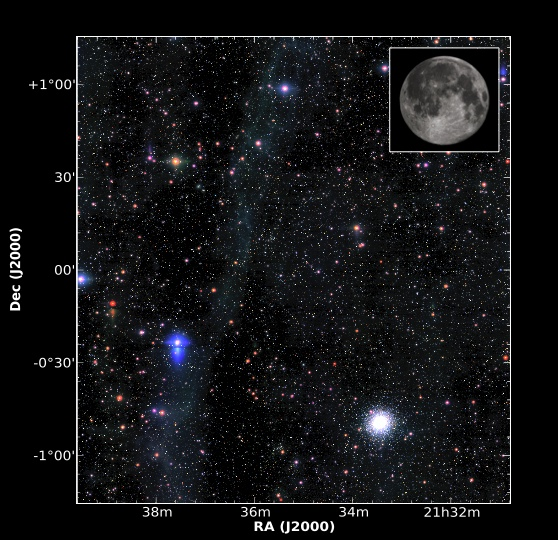
\includegraphics[width=1.0\hsize,clip]{DMStripe82.jpg}
\caption{
A small region in the vicinity of globular cluster M2, taken from a coadd of SDSS Stripe 82 data produced with LSST software stack prototypes. The coaddition employs a novel ``background matching" technique that improves background estimation and preserves the diffuse structures in the resulting coadd. The full coadd can be browsed at \url{http://moe.astro.washington.edu/sdss}.}
\label{Fig:DMStripe82}
\end{figure}


The LSST data management software has been prototyped for over eight
years. It has been exercised in eight data challenges, with increasing
degrees of complexity. Besides processing simulated LSST data
(\S~\ref{sec:imsim}), it has been used to process images from CFHTLS
and SDSS (Abazajian et al. 2009). As an example,
Figure~\ref{Fig:DMStripe82} shows a small region in the vicinity of M2
taken from a large coaddition of SDSS Stripe 82 data, generated with LSST
software stack prototypes.
\\

The LSST software stack is free software, licensed under the terms of the GNU General
Public License, Version 3. The stack
prototype code and documentation are available via \url{http://ls.st/ug}.
Its open source nature, an open development
process, attention to software engineering, a long-term project
commitment and a modular design that can be modified for use with
other cameras
may make it useful for the processing of imaging data beyond LSST.

\B{
\vskip 0.4in
\subsection{Simulating the LSST System}


Throughout its design, construction and commissioning, the LSST needs
to be able demonstrate that it can achieve the requirements laid out
in the Science Requirements Documents (SRD) given its design and
as-delivered components, that the system can be calibrated to the
required level of fidelity, that the data management software can
extract the appropriate astrophysical signals, and that this can be
achieved with sufficient efficiency such that the telescope can
complete its primary objectives within the ten years of its duration
(including surveying 18,000 sq degrees of the sky, and completing the
Deep Drilling Fields, see \S \ref{Sec:minisurveys}).


Realizing these objectives requires that the project can characterize
the performance of the LSST including the performance of the
opto-mechanical systems, the response of the detectors and their
electronics, and the capabilities of the analysis software. A
simulation framework provides such a capability; delivering a virtual
prototype LSST against which design decisions, optimizations
(including descoping), and trade studies can be evaluated (Connolly
et al.~2010).


The framework underlying the LSST simulations is designed to be
extensible and scalable (i.e. capable of being run on a single
processor or across many-thousand core compute clusters). It comprises
four primary components: a simulation of the survey scheduler
(\S~\ref{sec:opsim}),
databases of simulated astrophysical catalogs of stars, galaxies,
quasars and Solar System objects (\S~\ref{sec:catalogs}), a system for generating observations
based on the pointing of the telescope, and a system for generating
realistic LSST images of a given area of sky
(\S~\ref{sec:imsim}). Computationally intensive routines are written
in $C/C^{++}$ with the overall framework and database interactions
using $Python$.  The purpose of this design is to enable the
generation of a wide range of data products for use by the
collaboration; from all-sky catalogs used in simulations of the LSST
calibration pipeline, to studies of the impact of survey cadence on
recovering variability, to simulated images of a single LSST focal
plane.


\subsubsection{ The LSST Operations Simulator \label{sec:opsim}}

The LSST Operations Simulator was developed to enable a
detailed quantitative analysis of the various science tradeoffs described in
this paper. It contains detailed models of site conditions, hardware and
software performance, and an algorithm for scheduling observations which will,
eventually, drive the largely robotic observatory.
Observing conditions include a model for seeing derived from an extensive body
of on-site MASS/DIMM (Multi-Aperture Scintillation Sensor and Differential
Image Motion Monitor) measurements obtained during site selection and
characterization (see Fig.~\ref{Fig:seeing}). It not only reproduces the
observed seeing distribution, but includes
the auto-correlation spectrum of seeing with time over intervals from minutes
to seasons. Weather data are taken from ten years of hourly measurements at
nearby Cerro Tololo. The time history of site conditions is important if the
simulation is to faithfully reproduce a sequence of observations. Thus, for
example, the simulator correctly represents the variation of limiting
magnitude between pairs of observations used to detect NEOs and the
correlation between, for example, seasonal weather patterns and observing
conditions at any given point on the sky.  In addition, down time for
observatory maintenance is also included.

The signal-to-noise ratio of each
observation is determined using a sky background model which includes the dark
sky brightness in each filter, the effects of seeing and atmospheric
transparency, and a detailed model for scattered light from the moon and/or
twilight at each observation. The time taken to move from one observation to
the next is given by a detailed model of the camera, telescope, and dome. It
includes such effects as the acceleration/deceleration profiles employed in
moving the telescope, the dome, and the wind screen,
% in altitude, azimuth, camera rotator, dome azimuth, and wind/stray light screen altitude,
the time needed to damp vibrations excited by each slew,
cable wrap, the time taken for active optics lock and correction as a function of
slew distance, and the time for filter changes and focal plane readout.

Observations are scheduled by a ranking algorithm. After a given exposure, all
possible next observations are assigned a score which depends upon their locations, times,
and filters according to a set of scientific requirements which can vary with
time and location. For example, if an ecliptic field has been observed in the
$r$ band, the score for another $r$-band observation of the same field will
initially be quite low, but it will rise in time to peak about an hour after
the first observation, and decline thereafter. This algorithm results in
observations being acquired as pairs roughly an hour apart, which enables
efficient association of NEO detections. To ensure uniform
sky coverage, fields with fewer previous observations will be scored more
highly than those which have already been observed more frequently.

Once all possible next observations have been scored for scientific
priority, their scores are modified according to observing conditions
(e.g., seeing, airmass, and sky brightness) and to criteria such as
low slew time to move from the current position, time required to
change filters, etc. The highest-ranked observation is then performed,
and the cycle repeats. The result of a simulator run is a detailed
history of which locations on the sky were observed when, in what
filter, and with what sky background, seeing and other observing
conditions.  It takes a few days to produce a decade-long simulation
using an average PC.

\subsubsection{Catalog Generation}
\label{sec:catalogs}

The simulated astronomical catalogs are stored in an SQL
database. This base catalog is queried using sequences of observations
derived from the Operations Simulator. Each simulated
pointing provides a position and time of the observation together with
the appropriate sky conditions (e.g. seeing, moon phase and angle, sky
brightness and sky transparency). Positions of sources are propagated
to the time of observation (including proper motions for stars and
orbits for Solar System sources). Magnitudes and source counts are
derived using the atmospheric and filter response functions
appropriate for the airmass of the observation and after applying
corrections for source variability.  The resulting catalogs are then
formatted for either output to users, or fed into an image
simulator. Images are generated by ray-tracing individual photons
through the atmosphere, telescope and camera systems. Photons are
drawn from the spectral energy distributions that define the simulated
sources and ray-traced through the atmosphere and optical system
before conversion to electrons by simulating the camera physics.
Images are read out using a simulation of the camera electronics and
amplifier layout and formatted for ingestion into the LSST data
management system. All observing conditions, defined by the Operations
Simulator, are propagated through the catalog and image generation to
preserve fidelity and consistency between the derived catalogs and
images.

The current version of the LSST simulation framework incorporates
galaxies derived from an N-body simulation of a $\Lambda$CDM
cosmology, quasars/AGNs, stars that match the observed stellar
distributions within our Galaxy, asteroids generated from simulations
of our Solar System, and a 3-D model for Galactic extinction.  Stellar
sources are based on the Galactic structure models of Juri\'{c} et
al.~(2008) and include thin-disk, thick-disk, and halo star
components. The distribution and colors of the stars match those
observed by SDSS. Each star in the simulation is matched to a template
spectral energy distribution (SED). Kurucz (1993) model spectra are
used to represent main-sequence F, G, and K stars as well as RGB
stars, blue horizontal branch stars, and RR Lyrae variables.  SEDs for
white dwarf stars are taken from Bergeron et al.~(1995).  SEDs for M,
L, and T dwarfs are generated from a combination of spectral models
and by stacking spectra from the SDSS (e.g., Cushing et al.~2005,
Bochanski et al.~2007, Burrows et al.~2006, Petterson \& Hawley 1989,
Kowalski et al.~2010). The adopted metallicity for each star is based
on a model from Ivezi\'{c} et al.~(2008a), and proper motions are
based on the kinematic model of Bond et al.~(2010).  Light curve
templates are randomly assigned to a subset of the stellar population
so that variability may also be simulated. For Galactic reddening, a
value of $E(B-V)$ is assigned to each star using the three-dimensional
Galactic model of Amores \& Lepine (2005). To provide consistency with
the modeling of extragalactic fluxes in the simulations, the dust model in the Milky Way integrated
to 100 kpc is re-normalized to match the Schlegel et al.~(1998) dust maps.

Galaxy catalogs are derived from the Millennium simulations of de
Lucia et al.~(2006).  These models extend pure dark matter N-body
simulations to include gas cooling, star formation, supernovae and
AGN, and are designed to reproduce the observed colors, luminosities,
and clustering of galaxies as a function of redshift. To generate the
LSST simulated catalogs, a light cone, covering redshifts $0<z<6$, was
constructed from 58 simulation snapshots 500h$^{-1}$Mpc on a side. This
light cone extends to a depth of approximately $r=28$ and covers a
4.5$^\circ$$\times$4.5$^\circ$ footprint on the sky. Replicating this
catalog across the sky simulates the full LSST footprint. As with the
stellar catalog, an SED is fit to the colors of each source using
Bruzual \& Charlot (2003) spectral synthesis models. These fits are
undertaken separately for the bulge and disk components and, for the
disk, include inclination-dependent reddening. Morphologies are
modeled using two Sersic profiles. The bulge-to-disk ratio and disk
scale lengths are taken from de Lucia et al.~(2006). Half-light radii
for bulges are estimated using the empirical absolute-magnitude
vs. half-light radius relation given by Gonzalez et
al.~(2009). Comparisons between the redshift and number-magnitude
distributions of the simulated catalogs with those derived from deep
imaging and spectroscopic surveys showed that the de Lucia et
al.~models under-predict the density of sources at faint magnitudes
and high redshifts. To correct for these effects, sources are cloned
in magnitude and redshift space until their densities reflect the
average observed properties.

Quasar/AGN catalogs are generated using the Bongiorno et al.~(2007)
luminosity function for $M_B < -15$, over an area of 100
deg$^2$. Their observed SEDs are generated using a composite
rest-frame spectrum derived from SDSS data by Vanden Berk et
al.~(2001). The host galaxy is selected to have the closest match to
the preferred stellar mass and color at the AGN's redshift, following
the results from Xue et al.~(2010).  Each galaxy hosts at most one
AGN, and no explicit distinction is made between low-luminosity AGN and
quasars that dramatically outshine their host galaxies. The light
curve for each AGN is generated using a damped random walk model and
prescriptions given by MacLeod et al.~(2010).

Asteroids are simulated using the Solar System models of Grav et
al.~(2007). They include: Near Earth Objects (NEOs), Main Belt
Asteroids, the Trojans of Mars, Jupiter, Saturn, Uranus, and Neptune,
Trans Neptunian Objects, and Centaurs. Spectral energy distributions
are assigned using the C and S type asteroids of DeMeo et
al.~(2009). Positions for the 11 million asteroids in the simulation
are stored within the base catalog (sampled once per night for the ten
year duration of the LSST survey). We generate
accurate ephemerides of all asteroids falling within a given LSST
point using the $PyOrb$ software package (Granvik et
al.~2009). With typically 8000 sources per LSST field of view, this
procedure significantly reduces the computational resources
required to simulate asteroid ephemerides.



\subsubsection{Image Simulations}
\label{sec:imsim}

The framework described above provides a parametrized view of the sky
above the atmosphere. To generate images, photons are drawn from the
spectral energy distribution of each source (scaled to the appropriate
flux density based on the apparent magnitude of a source and
accounting for the spatial distribution of light for extended
sources). Each photon is ray-traced through the atmosphere, telescope
and camera to generate a CCD image. The atmosphere is modeled using a
Taylor frozen screen approximation (with the atmosphere described by
six layers). The density fluctuations within these screens are
described by a Kolmogorov spectrum with an outer scale (typically 10m
to 200m). All screens move during an exposure with velocities derived
from NOAA measurements of the wind velocities above the LSST site in
Chile.  Typical velocities are on the order of 20 m s$^{-1}$, and are
found to have a seasonable dependence that is modeled when generating
the screens. Each photon's trajectory is altered due to refraction as
it passes through each screen.


\begin{figure*}
\centerline{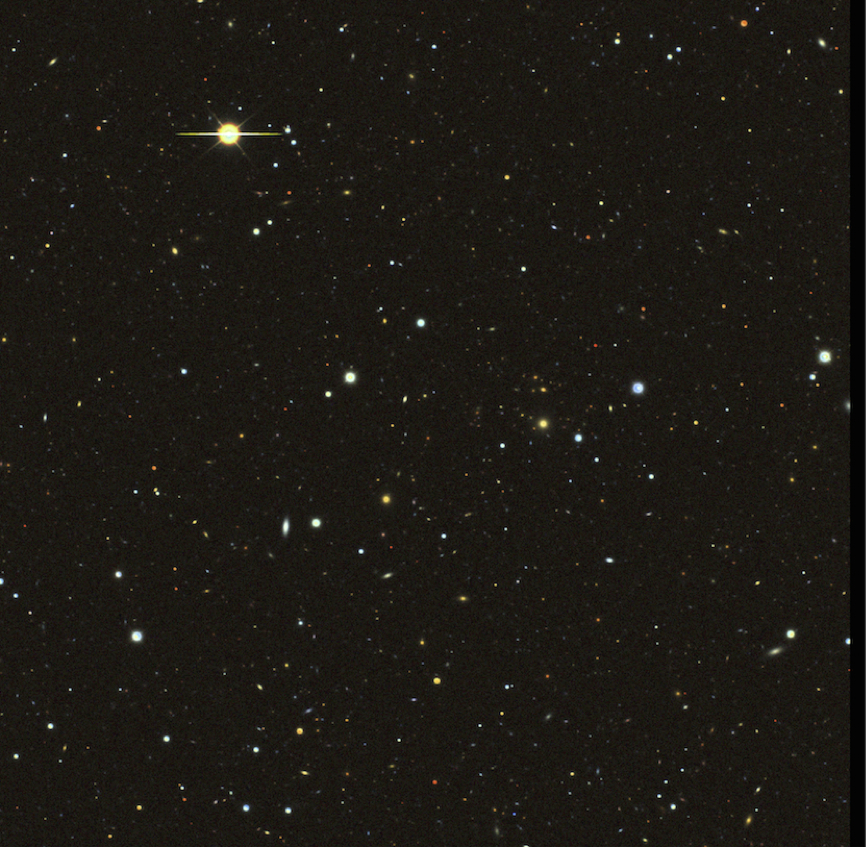
\includegraphics[width=0.98\textwidth,clip]{chip2014.jpg}}
%\vskip -1in
\caption{ A simulated image of a single LSST CCD (covering a
  $13.3\times13.3$ arcmin$^2$ region of the sky). The image is a color
  composite (Lupton et al.~2004) from a set of 30 second $gri$ visits.}
\label{Fig:ImSimExample}
\end{figure*}




After the atmospheric refraction, photons are reflected and refracted
by the optical surfaces within the telescope and camera. The mirrors
and lenses are simulated using geometric optics techniques in a fast
ray-tracing algorithm and all optical surfaces include a spectrum of
perturbations based on design tolerances. Each optic moves according
to its six degrees of freedom within tolerances specified by the LSST
system. Fast techniques for finding intercepts on the aspheric surface
and altering the trajectory of a photon by reflection or
wavelength-dependent refraction have been implemented to optimize the
efficiency of the simulated images. Wavelength and angle-dependent
transmission functions are incorporated within each of these
techniques, including simulation of the telescope spider.

Ray tracing of the photons continues into the silicon of the
detector. The conversion probability, refraction as a function of
wavelength and temperature, and charge diffusion within the silicon
are modeled for all photons. Photons are pixelated and the readout
process simulated including blooming, charge saturation, charge
transfer inefficiency, gain and offsets, hot pixels and columns, and
QE variations. The sky background is added as a post-processing step,
and includes Rayleigh scattering of the moon's light, based on SEDs
for the full moon and the dark sky. The background is vignetted
according to the results of ray-trace simulations.

The simulator generates $\sim$300,000 photons per second on an average
workstation. To produce simulated data corresponding to a night of
regular LSST operations requires approximately 0.5-1 million CPU hours
and, therefore, necessitates the use of large compute clusters.  An
example of a simulated image is shown in Fig.~\ref{Fig:ImSimExample}.
}
